\documentclass{article}[12pt]

% if you need to pass options to natbib, use, e.g.:
\PassOptionsToPackage{numbers, sort&compress}{natbib}
% before loading nips_2017
%
% to avoid loading the natbib package, add option nonatbib:
% \usepackage[nonatbib]{nips_2017}

%\usepackage{nips_2017}

% to compile a camera-ready version, add the [final] option, e.g.:
% \usepackage[final]{nips_2017}

\usepackage[utf8]{inputenc} % allow utf-8 input
\usepackage[T1]{fontenc}    % use 8-bit T1 fonts
\usepackage[pagebackref]{hyperref}       % hyperlinks
\usepackage{url}            % simple URL typesetting
\usepackage{booktabs}       % professional-quality tables
\usepackage{amsfonts}       % blackboard math symbols
\usepackage{nicefrac}       % compact symbols for 1/2, etc.
\usepackage{microtype}      % microtypography
%\usepackage{algorithm}
%\usepackage{algorithmic}
\usepackage{algpseudocode}
\usepackage{amsthm,amssymb,amsopn,amsmath}
\usepackage{graphicx} % more modern
%\usepackage{epsfig} % less modern
\usepackage{graphicx}
\usepackage{subcaption}
\usepackage{wrapfig}
\usepackage{natbib}
\usepackage{authblk}
%\usepackage[nonatbib]{nips_2016}
\newtheorem{assumption}{Assumption}
\newtheorem{define}{Definition}
\newtheorem{thm}{Theorem}
\newtheorem{lem}{Lemma}
\newtheorem{coro}{Corollary}
\newcommand*\samethanks[1][\value{footnote}]{\footnotemark[#1]}

\title{Counterfactual Fairness}
\author[1,2]{Matt J. Kusner\thanks{Equal contribution, author order decided randomly.}}
\author[1,3]{Joshua R. Loftus\samethanks}
\author[1,4]{Chris Russell\samethanks}
\author[1,5]{Ricardo Silva}
\affil[1]{Alan Turing Institute}
\affil[2]{University of Warwick}
\affil[3]{University of Cambridge}
\affil[4]{University of Edinburgh}
\affil[5]{University College London}
%\author{Matt J. Kusner\footnote{}, Joshua R. Loftus, Chris Russell, Ricardo Silva}
\date{}
%\newcommand\independent{\protect\mathpalette{\protect\independenT}{\perp}}
\def\independenT#1#2{\mathrel{\rlap{$#1#2$}\mkern2mu{#1#2}}}
\newcommand\cff{{\sc cff}}
%\footnote{Equal contribution, author order decided randomly.}
% Code blocks%
\usepackage{listings}
\usepackage{color}

\newcommand\independent{\protect\mathpalette{\protect\independenT}{\perp}}

% Code blocks%
\usepackage{listings}
\usepackage{color}

\definecolor{dkgreen}{rgb}{0,0.6,0}
\definecolor{gray}{rgb}{0.5,0.5,0.5}
\definecolor{mauve}{rgb}{0.58,0,0.82}

\lstset{frame=tb,
  language=matlab,
  aboveskip=3mm,
  belowskip=3mm,
  showstringspaces=false,
  columns=flexible,
  basicstyle={\small\ttfamily},
  numbers=none,
  numberstyle=\tiny\color{gray},
  keywordstyle=\color{blue},
  commentstyle=\color{dkgreen},
  stringstyle=\color{mauve},
  breaklines=true,
  breakatwhitespace=true,
  tabsize=3
}


\begin{document}
\maketitle

% this must go after the closing bracket ] following \twocolumn[ ...

% This command actually creates the footnote in the first column
% listing the affiliations and the copyright notice.
% The command takes one argument, which is text to display at the start of the footnote.
% The \icmlEqualContribution command is standard text for equal contribution.
% Remove it (just {}) if you do not need this facility.

%\printAffiliationsAndNotice{}  % leave blank if no need to mention equal contribution
%\printAffiliationsAndNotice{\textsuperscript{*}Equal contribution, author order decided randomly}
%\icmlEqualContribution}
%%\icmlEqualContribution} % otherwise use the standard text.
%\footnotetext{hi}

\begin{abstract} 
% fairness is important
  Machine learning can impact people with legal or ethical
  consequences when it is used
  %has matured to the point to where it is now being   considered
  to automate decisions in areas such as insurance, lending, hiring,
  and predictive policing.  In many of these scenarios,
  previous decisions have been made that are unfairly biased against
  certain subpopulations, for example those of a particular race, gender, or
  sexual orientation.  Since this past data may be biased,
  machine learning predictors must account for this to avoid
  perpetuating or creating discriminatory practices.
  In this paper, we develop a framework for modeling fairness
  using tools from causal inference. Our definition of
  \emph{counterfactual fairness} captures the
  intuition that a decision is fair towards an individual if it 
  the same in (a) the actual world and (b) a counterfactual world
  where the individual belonged to a different demographic
  group. We demonstrate our framework on a real-world problem of fair
  prediction of success in law school.
  %demonstrate our framework on two real-world problems: fair
  %prediction of law school success, and fair modeling of an
  %individual's criminality in policing data.
\end{abstract} 

\section{Contribution}
\label{sec:introduction}
%!TEX root=ricardo_draft.tex
% ml is now everywhere
Machine learning has spread to fields as diverse as credit scoring
\cite{khandani2010consumer}, crime prediction
\cite{brennan2009evaluating}, and loan assessment
\cite{mahoney2007method}. Decisions in these areas may have ethical or
legal implications, so it is necessary for the modeler to think beyond
the objective of maximizing prediction accuracy and consider the
societal impact of their work.
% in these new ml fields, we cannot discriminate
% discrimination can happen in multiple ways
% - direct discrimination
For many of these applications, it is crucial to ask if the
predictions of a model are \emph{fair}.  Training data can contain
unfairness for reasons having to do with historical prejudices or
other factors outside an individual's control.
% For instance, imagine a bank
% wishes to predict if an individual should be given a loan to buy a
% house. The bank wishes to use historical repayment data, alongside
% individual data. If they simply learn a model that predicts whether
% the loan will be paid back, it may unjustly favor applicants of
% particular subgroups, due to past and present prejudices.
In 2016, the Obama administration released a
report\footnote{https://obamawhitehouse.archives.gov/blog/2016/05/04/big-risks-big-opportunities-intersection-big-data-and-civil-rights}
which urged data scientists to analyze ``how technologies can
deliberately or inadvertently perpetuate, exacerbate, or mask
discrimination."

There has been much recent interest in designing algorithms that make
fair predictions
\cite{hardt2016equality,dwork2012fairness,joseph2016rawlsian,kamishima2011fairness,zliobaite2015survey,zafar2016fairness,zafar2015learning,grgiccase,kleinberg:17,calders2010three,kamiran2012data,bolukbasi2016man,kamiran2009classifying,zemel2013learning,louizos2015variational}.
% Most
% of these works focus on formalizing fairness into a numeric
% definition and satisfying it with customized algorithms.
In large part, the literature has focused on formalizing fairness into
quantitative definitions and using them to solve a discrimination
problem in a certain dataset. Unfortunately, for a practitioner,
law-maker, judge, or anyone else who is interested in implementing
algorithms that control for discrimination, it can be difficult to
decide {\em which} definition of fairness to choose for the task at
hand. Indeed, we demonstrate that depending on the relationship
between a protected attribute and the data, certain definitions of
fairness can actually \emph{increase discrimination}.

% we propose a way to model data that allows a practitioner to assess what definitions of fairness are right for the problem at hand, and algorithms to ensure fairness
% OR
% we propose a way to interpret fairness...
% a) relationship between fairness and causality
% b) use pearl's models
% c) having an explicit model allows us to test fairness with the assumptions laid bare
% tension: Pearl already talks about discrimination, so we aren't really inventing new models. Are we even new in using these models to talk about fairness? Maybe... Pearl talks about variables that we might want to compute counterfactuals for in order to see if discrimination is happening.  
% Our proposal is:
% - situate a sensitive variable in a graph (not new).
% - Look at old definitions and see if anything bad could happen (new). 
% - Then define counterfactual fairness (new). 
% - Modeling helps us see where the weaknesses are in our assumptions and definitions (maybe not new)
% We don't want to see if every definition is counterfactually fair because then we're like everyone else, saying our definition is best
% 
% In this work,

In this paper, we introduce the first explicitly causal approach to
address fairness.  Specifically, we leverage the causal framework of
\citet{pearl2009causal} to model the relationship between protected
attributes and data. We describe how techniques from causal inference
can be effective tools for designing fair algorithms and argue, as in
\citet{dedeo2014wrong}, that it is essential to properly address
causality in fairness. In perhaps the most closely related prior work,
\citet{johnson2016impartial} make similar arguments but from a
non-causal perspective. An alternative use of causal modeling in
the context of fairness is introduced independently by \citep{kilbertus:17}.

In Section \ref{sec:background}, we provide a summary of basic
concepts in fairness and causal modeling. In Section
\ref{sec:count_fair}, we provide the formal definition of
\emph{counterfactual fairness}, which enforces that a distribution
over possible predictions for an individual should remain unchanged in
a world where an individual's protected attributes had been different
in a causal sense. In Section \ref{sec:methods}, we describe an
algorithm to implement this definition, while distinguishing it from
existing approaches.  In Section \ref{sec:experiments}, we illustrate
the algorithm with a case of fair assessment of law school success.

%%%%%%% ICML TEXT
%In this paper, we introduce the first explicitly formal causal model
%approach for casting problems of fair predictions with explicit
%counterfactual assumptions. We describe how techniques from causal
%inference can be effective tools for designing fair algorithms and
%argue, as in \citet{dedeo2014wrong}, that it is essential to properly
%address causality.  Specifically, we leverage the causal framework of
%\citet{pearl2009causal} to model the relationship between sensitive
%attributes and data. Our contributions are as follows:
%\begin{enumerate}
%    \item We model questions of fairness within a causal
%      framework. This allows us to directly model \emph{how}
%      unfairness affects the data at hand.
%    \item We introduce \emph{counterfactual fairness}, which enforces
%      that a distribution over possible predictions for an individual
%      should remain unchanged, in a world where an individual's
%      sensitive attribute had been different from birth.
%    \item We analyze how enforcing existing definitions of fairness
%      for different data may correspond or be in conflict with
%      counterfactual fairness. In particular, we show that depending
%      on the underlying state of the world some definitions of
%      fairness may be inappropriate.
%    \item We devise techniques for learning predictors that are
%      counterfactually fair and demonstrate their use in several
%      examples.
%\end{enumerate}
%%%%%%%% END ICML TEXT

%We demonstrate that by explicitly representing fairness within a causal model it becomes easy to critique different definitions of fairness as well the prediction methods that aim to accomplish these notions of fairness.




% RETHINK SPIN, ALWAYS RETHINK

%%% Local Variables:
%%% mode: latex
%%% TeX-master: "ricardo_draft"
%%% End:


\section{Background}
\label{sec:background}
%!TEX root=ricardo_draft.tex
% We begin by describing the problem of fair prediction and introduce three of the most popular definitions developed for this task.  We then give a brief overview of causal modeling which will act as our `tool-kit' for modeling and defining fairness.

% \subsection{Fairness}
% Consider a scenario in which predictions must be fair. For instance, imagine a university in the United States (US) would like to know how successful an applicant is going to be after graduation, call this $Y$, given their current incoming features $X$ such as test scores, grade-point average (GPA). To predict success a modeler is given a dataset of $n$ applications with features $\{X^{(1)}, \ldots, X^{(n)} \}$ and measures of graduation success $\{Y^{(1)}, \ldots, Y^{(n)}\}$. However, historically  student admission \cite{kane1998racial,kidder2000portia} in universities in the US suffered from racial and gender biases. Thus, in addition we are given demographic and gender information for each individual $\{A^{(1)}, \ldots, A^{(n)}\}$ that we will use to ensure our model is fair.

% What does it mean for a model to be fair?  There has
% been a wealth of recent works aimed at answering this. A few popular
% definitions are (a) Fairness Through Unawareness
% (FTU)~\citep{dwork2012fairness,grgiccase}, (b) Demographic Parity (DP)
% \citep{kleinberg2016inherent}, (c) Equal Opportunity (EO)
% \citep{kleinberg2016inherent}, and (d) Individual Fairness (IF). These
% are defined as follows:

% \begin{define}[Fairness Through Unawareness (FTU)]
%   An algorithm is fair so long as the sensitive attribute $A$ is not
%   explicitly used in the decision-making process. Any mapping
%   $\hat{Y}: X \rightarrow Y$ that excludes $A$ (or other attributes
%   considered  unfair, see \citet{grgiccase}) satisfies this
%   definition.
% \end{define}

% \begin{define}[Demographic Parity (DP)]
% An algorithm is fair if its predictions are independent of the sensitive attributes $A$ across the population. A prediction $\hat{Y}$ satisfies this definition if, 
% \begin{align}
% P(\hat{Y} | A = 0) = P(\hat{Y} | A = 1). \nonumber
% \end{align}
% \end{define}

% \begin{define}[Equal Opportunity (EO)]
% An algorithm is fair if it is equally accurate for each value of the sensitive attribute $A$. A prediction $\hat{Y}$ satisfies this if,
% \begin{align}
% P(\hat{Y}=1 | A=0,Y=1) = P(\hat{Y}=1 | A=1,Y=1). \nonumber
% \end{align}
% \end{define}



%\subsection{Causal Models and Counterfactuals}
\label{subsec:cmc}
We follow the framework of \citet{pearl:00}, and define a causal
model as a triple $(U, V, F)$ of sets such that
%
\begin{itemize}
\item $U$ is a set of {\bf background} variables\footnote{These are
  sometimes called {\bf exogenous variables}, but the fact that members of $U$
  might depend on each other is not relevant to what follows.}, which are generated by factors
outside of our potential control, and do not depend on any protected attributes $A$;
\item $V$ is a set of {\bf endogenous} variables, where each member is determined by
  other variables in $U \cup V$;
\item $F$ is a set of functions $\{f_1, \dots, f_n\}$, one for each $V_i \in V$, such
that $V_i = f_i(pa_i, U_{pa_i})$, $pa_i \subseteq V \backslash
\{V_i\}$ and $U_{pa_i} \subseteq U$. Such equations are also known as
{\bf structural equations} \citep{bol:89}.
\end{itemize}
%
The notation ``$pa_i$'' refers to the ``parents'' of $V_i$ and is motivated by the assumption that the
model factorizes according to a directed acyclic graph (DAG). That is, we can
define a directed graph ${\mathcal G}=(U \cup V, \mathcal E )$ where each node is an
element of $U \cup V$, and each edge from some $Z \subseteq U \cup V$ to $V_i$ indicates that $Z \in pa_i \cup U_{pa_i}$. By construction, $\mathcal G$ is
acyclic.

The model is causal in that, given a distribution $p(U)$
over the background variables $U$, you can derive the distribution of
a subset $Z \subseteq V$ following an {\bf intervention} on the
complementary subset $V\setminus Z$.  Here,
an {\bf intervention} on the variable $V_i$ of value $v$ refers to the substitution of
equation $V_i = f_i(pa_i, U_{pa_i})$ with the equation $V_i =
v$. This captures the idea of an agent, external to the
system, modifying it by forcefully assigning value $v$ to $V_i$. This occurs in a randomized controlled trials where the value
of $V_i$ is overridden by a treatment setting it to $v$, a value
chosen at random, and thus independent of any other causes.% of the
%system. % The do-calculus of \citet{pearl:00} provides a way to identify
% features of interventional distributions %, where possible,
% using only estimates of the joint distribution of $V$ and knowledge of
% the causal DAG.

In contrast with the independence constraints given by a DAG, the full
specification of $F$ requires much stronger assumptions but also leads
to much stronger claims. In particular, it allows for the
calculation of {\bf counterfactual} quantities. % Without going into a
% detailed coverage of the topic
In brief, consider the following counterfactual
statement, ``the value of $Y$ if $Z$ had taken value $z$'', for two endogenous
variables $Z$ and $Y$ in a causal model. By assumption, the state of
any endogenous variable is fully determined by
the background variables and structural equations. The counterfactual is
modeled as the solution for $Y$ for a given $U = u$ where the equations
for $Z$ are replaced with $Z \!=\! z$.  We denote it by $Y_{Z \leftarrow z}(u)$
\cite{pearl:00}, and sometimes as $Y_z$ if the context of the notation is clear.

Counterfactual inference, as specified by a causal model $(U, V, F)$ given evidence $W$,
is the computation of probabilities
$P(Y_{Z \leftarrow z}(U)\ |\ W \!=\! w)$, where $W$, $Z$ and $Y$ are
subsets of $V$. Inference proceeds in three steps, as explained in
more detail in Chapter 4 of \citet{pearl:16}:
\begin{enumerate}
\item Abduction: for a given prior on $U$, compute the posterior
  distribution of $U$ given the evidence $W = w$;
\item Action: substitute the equations for $Z$ with the interventional
  values $z$, resulting in the modified set of equations $F_z$;
\item Prediction: compute the implied distribution on the remaining
  elements of $V$ using $F_z$ and the posterior $P(U\ | W = w)$.
\end{enumerate}



%%% Local Variables:
%%% mode: latex
%%% TeX-master: "ricardo_draft"
%%% End:


%\section{Background}
%\label{sec:related}
%% !TEX root=ricardo_draft.tex
% binary classification
There has been a wealth of recent work towards fair machine learning
algorithms. In large part, these methods have focussed (and reasonably
so) on binary classification with a binary sensitive attributes
(CITE). A concurrent goal of these works was to construct a working
definition of fairness (or unfairness) that could be evaluated and
optimized. These include fairness through unawareness/disparate
treatment\cite{grgiccase,zafar2016fairness}, demographic
parity/disparate impact \cite{zafar2015learning}, individual fairness
\cite{dwork2012fairness,zemel2013learning,louizos2015variational,joseph2016rawlsian},
equality of opportunity/disparate
mistreatment~\cite{hardt2016equality,zafar2016fairness}.

A variety of algorithmic approaches to achieving fairness have been proposed. Most similar to our work is \cite{zemel2013learning} (I have no idea which reference we're going for here).      




% finding a latent U

% orthogonal features


%%% Local Variables:
%%% mode: plain-tex
%%% TeX-master: "ricardo_draft"
%%% End:


%\section{Causal Models and Counterfactuals}
%\label{sec:background}
%%!TEX root=ricardo_draft.tex
% We begin by describing the problem of fair prediction and introduce three of the most popular definitions developed for this task.  We then give a brief overview of causal modeling which will act as our `tool-kit' for modeling and defining fairness.

% \subsection{Fairness}
% Consider a scenario in which predictions must be fair. For instance, imagine a university in the United States (US) would like to know how successful an applicant is going to be after graduation, call this $Y$, given their current incoming features $X$ such as test scores, grade-point average (GPA). To predict success a modeler is given a dataset of $n$ applications with features $\{X^{(1)}, \ldots, X^{(n)} \}$ and measures of graduation success $\{Y^{(1)}, \ldots, Y^{(n)}\}$. However, historically  student admission \cite{kane1998racial,kidder2000portia} in universities in the US suffered from racial and gender biases. Thus, in addition we are given demographic and gender information for each individual $\{A^{(1)}, \ldots, A^{(n)}\}$ that we will use to ensure our model is fair.

% What does it mean for a model to be fair?  There has
% been a wealth of recent works aimed at answering this. A few popular
% definitions are (a) Fairness Through Unawareness
% (FTU)~\citep{dwork2012fairness,grgiccase}, (b) Demographic Parity (DP)
% \citep{kleinberg2016inherent}, (c) Equal Opportunity (EO)
% \citep{kleinberg2016inherent}, and (d) Individual Fairness (IF). These
% are defined as follows:

% \begin{define}[Fairness Through Unawareness (FTU)]
%   An algorithm is fair so long as the sensitive attribute $A$ is not
%   explicitly used in the decision-making process. Any mapping
%   $\hat{Y}: X \rightarrow Y$ that excludes $A$ (or other attributes
%   considered  unfair, see \citet{grgiccase}) satisfies this
%   definition.
% \end{define}

% \begin{define}[Demographic Parity (DP)]
% An algorithm is fair if its predictions are independent of the sensitive attributes $A$ across the population. A prediction $\hat{Y}$ satisfies this definition if, 
% \begin{align}
% P(\hat{Y} | A = 0) = P(\hat{Y} | A = 1). \nonumber
% \end{align}
% \end{define}

% \begin{define}[Equal Opportunity (EO)]
% An algorithm is fair if it is equally accurate for each value of the sensitive attribute $A$. A prediction $\hat{Y}$ satisfies this if,
% \begin{align}
% P(\hat{Y}=1 | A=0,Y=1) = P(\hat{Y}=1 | A=1,Y=1). \nonumber
% \end{align}
% \end{define}



%\subsection{Causal Models and Counterfactuals}
\label{subsec:cmc}
We follow the framework of \citet{pearl:00}, and define a causal
model as a triple $(U, V, F)$ of sets such that
%
\begin{itemize}
\item $U$ is a set of {\bf background} variables\footnote{These are
  sometimes called {\bf exogenous variables}, but the fact that members of $U$
  might depend on each other is not relevant to what follows.}, which are generated by factors
outside of our potential control, and do not depend on any protected attributes $A$;
\item $V$ is a set of {\bf endogenous} variables, where each member is determined by
  other variables in $U \cup V$;
\item $F$ is a set of functions $\{f_1, \dots, f_n\}$, one for each $V_i \in V$, such
that $V_i = f_i(pa_i, U_{pa_i})$, $pa_i \subseteq V \backslash
\{V_i\}$ and $U_{pa_i} \subseteq U$. Such equations are also known as
{\bf structural equations} \citep{bol:89}.
\end{itemize}
%
The notation ``$pa_i$'' refers to the ``parents'' of $V_i$ and is motivated by the assumption that the
model factorizes according to a directed acyclic graph (DAG). That is, we can
define a directed graph ${\mathcal G}=(U \cup V, \mathcal E )$ where each node is an
element of $U \cup V$, and each edge from some $Z \subseteq U \cup V$ to $V_i$ indicates that $Z \in pa_i \cup U_{pa_i}$. By construction, $\mathcal G$ is
acyclic.

The model is causal in that, given a distribution $p(U)$
over the background variables $U$, you can derive the distribution of
a subset $Z \subseteq V$ following an {\bf intervention} on the
complementary subset $V\setminus Z$.  Here,
an {\bf intervention} on the variable $V_i$ of value $v$ refers to the substitution of
equation $V_i = f_i(pa_i, U_{pa_i})$ with the equation $V_i =
v$. This captures the idea of an agent, external to the
system, modifying it by forcefully assigning value $v$ to $V_i$. This occurs in a randomized controlled trials where the value
of $V_i$ is overridden by a treatment setting it to $v$, a value
chosen at random, and thus independent of any other causes.% of the
%system. % The do-calculus of \citet{pearl:00} provides a way to identify
% features of interventional distributions %, where possible,
% using only estimates of the joint distribution of $V$ and knowledge of
% the causal DAG.

In contrast with the independence constraints given by a DAG, the full
specification of $F$ requires much stronger assumptions but also leads
to much stronger claims. In particular, it allows for the
calculation of {\bf counterfactual} quantities. % Without going into a
% detailed coverage of the topic
In brief, consider the following counterfactual
statement, ``the value of $Y$ if $Z$ had taken value $z$'', for two endogenous
variables $Z$ and $Y$ in a causal model. By assumption, the state of
any endogenous variable is fully determined by
the background variables and structural equations. The counterfactual is
modeled as the solution for $Y$ for a given $U = u$ where the equations
for $Z$ are replaced with $Z \!=\! z$.  We denote it by $Y_{Z \leftarrow z}(u)$
\cite{pearl:00}, and sometimes as $Y_z$ if the context of the notation is clear.

Counterfactual inference, as specified by a causal model $(U, V, F)$ given evidence $W$,
is the computation of probabilities
$P(Y_{Z \leftarrow z}(U)\ |\ W \!=\! w)$, where $W$, $Z$ and $Y$ are
subsets of $V$. Inference proceeds in three steps, as explained in
more detail in Chapter 4 of \citet{pearl:16}:
\begin{enumerate}
\item Abduction: for a given prior on $U$, compute the posterior
  distribution of $U$ given the evidence $W = w$;
\item Action: substitute the equations for $Z$ with the interventional
  values $z$, resulting in the modified set of equations $F_z$;
\item Prediction: compute the implied distribution on the remaining
  elements of $V$ using $F_z$ and the posterior $P(U\ | W = w)$.
\end{enumerate}



%%% Local Variables:
%%% mode: latex
%%% TeX-master: "ricardo_draft"
%%% End:


\section{Counterfactual Fairness}
\label{sec:count_fair}
% !TEX root=ricardo_draft.tex
%%% TeX-master: "ricardo_draft"~\ref{figure.simple_models}
\begin{figure*}[th!]
\begin{center}
\vspace{-1ex}
\centerline{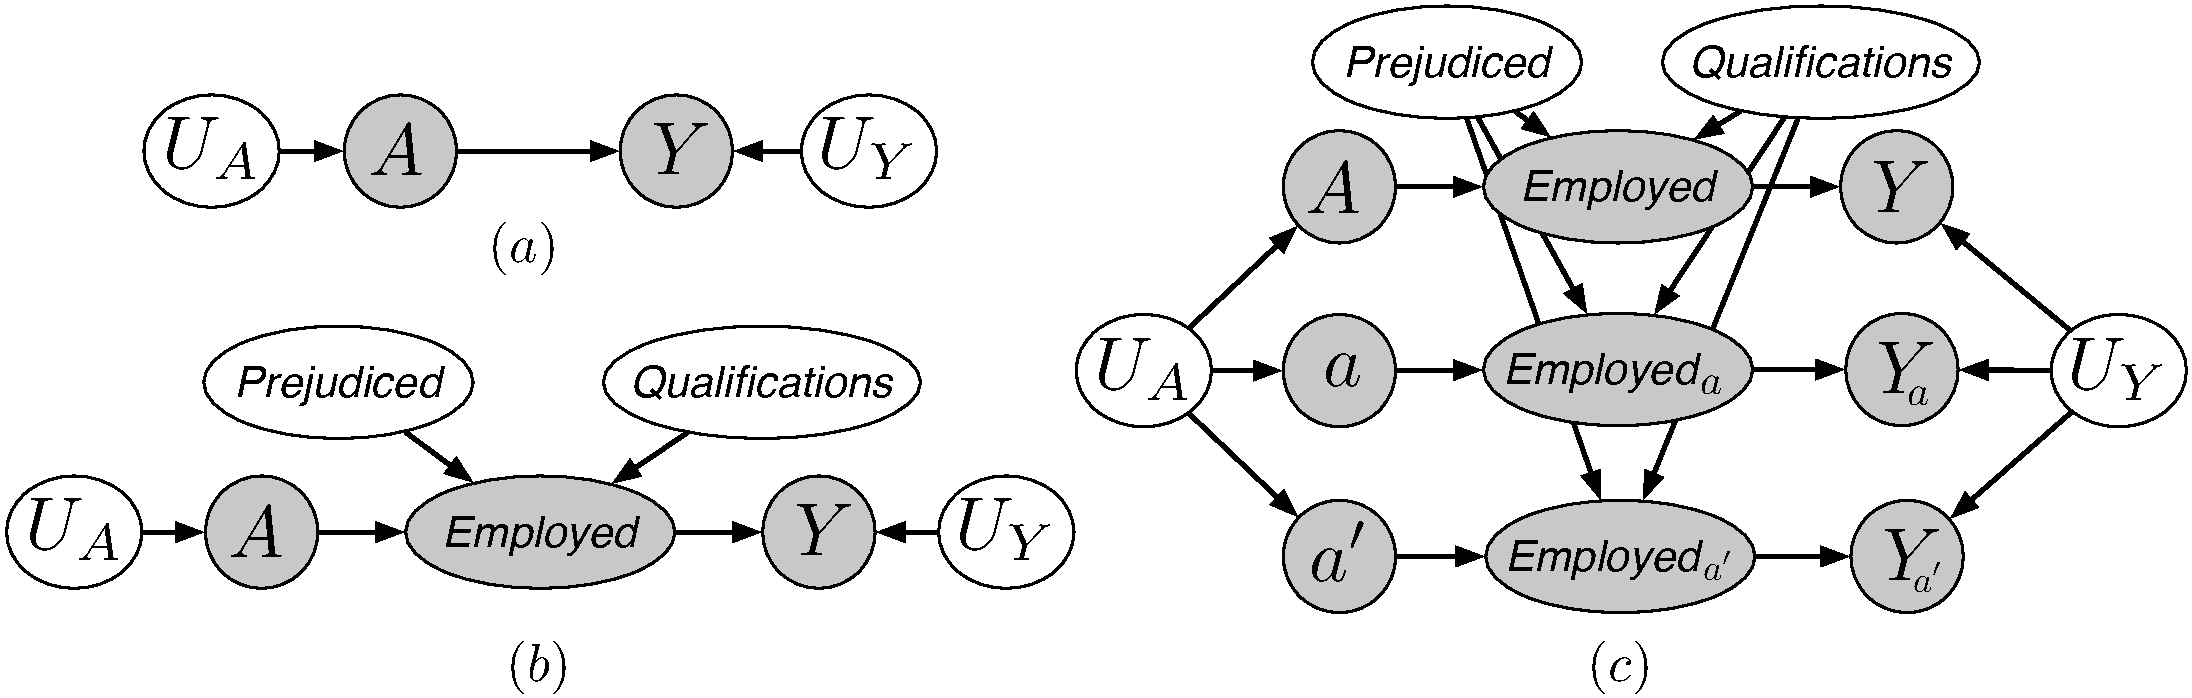
\includegraphics[width=\textwidth]{implications_fig.pdf}}
\vspace{-2ex}
\label{fig:ex1}
  \caption{(a) The graph corresponding to a causal model with $A$ being the protected attribute
    and $Y$ some outcome of interest, with background variables assumed to be independent.
    (b) Expanding the model to include an intermediate variable indicating whether the individual
    is employed with two (latent) background variables $\textbf{Prejudiced}$ (if the person  offering the job is prejudiced) and $\textbf{Qualifications}$ (a measure of the individual's qualifications). (c) A twin network representation of this system \citep{pearl:00}
    under two different counterfactual levels for $A$. This is created by copying nodes descending from $A$, which inherit unaffected parents from the factual world.\vspace{-5ex}}
\vspace{-2ex}
\end{center}
% \begin{center}
  % \begin{tabular}{c}
  %   Here, a graph $U_A \rightarrow A \rightarrow Y \leftarrow U_Y$
  %   (rearrange it spatially in any way you want (including this table).)\\ (a)\\ \\
  %   Here, a graph made of edges \\
  %   $A \leftarrow U_A$, $Employed \leftarrow \{A, Prejudiced, Qualifications\}$,
  %   $Y \leftarrow \{Employed, U_Y\}$. \\ (b)\\ \\
  %   Here, a twin network,
  %   $A \leftarrow U_A$, $Employed \leftarrow \{A, Prejudiced, Qualifications\}$,
  %   $Y \leftarrow \{Employed, U_Y\}$,\\
  %   $Employed_a \leftarrow \{a, Prejudiced, Qualifications\}$,
  %   $Y_a \leftarrow \{Employed_a, U_Y\}$,\\
  %   $Employed_{a'} \leftarrow \{a', Prejudiced, Qualifications\}$,
  %   $Y_{a'} \leftarrow \{Employed_{a'}, U_Y\}$,
  %   (``$a$'' and ``$a'$'' are two extra nodes too)\\.
  %   \\ (c)\\
  % \end{tabular}
  % \label{fig:ex1}
  % \caption{(a) The graph corresponding to a causal model with $A$ being the protected outcome
  %   and $Y$ some outcome of interest, with background variables assumed to be independent.
  %   (b) Expanding the model to include an intermediate variable indicating whether the individual
  %   is employed with two (latent) background variables $\textbf{Prejudiced}$ (whether the person in charge
  %   of offering the job is prejudiced) and $\textbf{Qualifications}$ (a measure of the qualifications of
  %   the individual). (c) A twin network representation of this system \citep{pearl:00}
  %   under two different counterfactual levels for $A$. The network is created by creating copies
  %   of nodes descending from $A$, which inherit parents from the factual world that have not
  %   been affected.}
% \end{center}
\end{figure*}


%\subsection{Definition}
%Formally, a variable $Y$ is said to be counterfactually fair with
%respect to a protected attribute $A$ if
Given a causal model $(U, V, F)$, let $A$ be a set of protected
attributes, $\hat Y$ a variable of interest which we will be the basis for
any decision making, and $W$ the set of complementary measurements such that
$W= V \setminus ( A \cup \{\hat Y\})$.
\begin{define}[Counterfactual fairness]
We say $\hat Y$ is {\bf counterfactually fair}
if under any context uniquely defined by $W = w$ and $A = a$,
  \label{eq:cf_definition}
\begin{align}
  &P(\hat Y_{A \leftarrow a\ }(U) = y\ |\ W = w, A = a)  =\nonumber\\ 
  &P(\hat Y_{A \leftarrow a'}(U) = y\ |\ W = w, A = a), 
\end{align}
for all $y$ and for any value $a'$ attainable by $A$.
\end{define}
%Simply put,
The above statement captures the idea that any decision based on the
conditional distribution of $\hat Y$ would have been the same had $A$ been
different, given the full implications of $A$ having always been different.
We can also see $\hat Y$ as satisfying ``counterfactual exchangeability''
under this model.
%This definition substantially differs from Fairness Through
%Unawareness, as it considers the influence of attributes such as race
%on other measured variables.

An associated concept of causal fairness appears as Example 4.4.4 in
\citet{pearl:16}. There, the authors condition instead on $W$, $A$,
and the observed realization of $\hat Y$, and calculate the
probability of the counterfactual realization differing from the
factual\footnote{The result is an expression called the ``the
  probability of sufficiency'' for $A$, capturing the notion that
  switching $A$ to a different value would be sufficient to change
  $\hat Y$ with some probability.}. This example conflates the
recorded decision $\hat Y$ with the information $Y$ on which we should
ideally base our decision making, a difference which we maintain.  Our
framing makes the connection to other existing machine learning
methods more explicit, as we discuss in Section \ref{sec:methods}.
Evidence used to determine the state of background variables $U$
should come from $A$ and $W$ alone, as in many setups we wish to
predict some $Y$ as $\hat Y$, when $Y$ is unavailable at any point in
our inference.

% We also emphasize that counterfactual fairness is an individual-level
% definition. This is substantially different from the notion of ``causal independence''
% as discussed in Section 4.3.1 of \cite{pearl:16}. Causal independence
% % requires
% % \begin{align}
% %   &P(\hat Y = y\ |\ do(A = a), W = w) =\nonumber\\ 
% %   &P(\hat Y = y\ |\ do(A = a'), W = w),
% % \end{align}
% % which
% entails comparing different units that happen to share the
% same ``treatment'' and coincide on values of $W$, while
% counterfactual fairness concerns the variation possible within an
% individual depending on their value of $a$ and the descendents of
% $A$ in the causal graph.
We also emphasize that counterfactual fairness is an
individual-level definition. This is substantially different
from comparing different units that happen to share the
same ``treatment'' and coincide on values of $X$, as discussed in
Section 4.3.1 of \citep{pearl:16}. Here, differences in the value
of $X$ must be caused by variations on $A$ only.

\subsection{Implications}
%
As discussed by \citet{halpern:16}, it is unproductive to debate
if a particular counterfactual definition is the ``correct'' one
to satisfy socially constructed concepts such as blame and responsibility.
The same applies to fairness. Instead, we discuss the
implications of definition \eqref{eq:cf_definition} and some choices
that arise in its application.

First, we wish to make explicit the difference between $\hat Y$, the
variable which we use for fair decisions, and $Y$, the related state
generated by an unfair world. For instance, $Y$ could be an indicator
of whether a client defaults on a loan, while $\hat Y$ is the actual
decision of giving the loan. Consider the DAG $A \rightarrow Y$ for a
causal model where $V = \{A, Y\}$, and in Figure \ref{fig:ex1}(a) the
DAG with explicit inclusion of set $U$ and assumptions about
independence of background variables. Assume $Y$ is an objectively
ideal measure to be used in decision making, such as a binary
indicator that the individual defaults on a loan. In this setup, we
postulate that the mechanism $f_Y(A, U)$ is unfair, with the arrow
$A \rightarrow Y$ being the result of a world that punishes
individuals in a way that is out of their control. Figure
\ref{fig:ex1}(b) shows a more fine-grained theoretical model, where
the path is mediated by a measure of whether the person is employed,
which is itself caused by two background factors: one representing
whether the person offering jobs is prejudiced, and one related to
their qualifications. Using the information about employment will
result in unfair predictions if employment is partially the result of
prejudice.

In the world  postulated by this example 
$A$ is a cause of defaulting, even if mediated by other
variables. The counterfactual fairness principle however forbids us
from using $Y$: using the twin network construction of
\citet{pearl:00}, we see in Figure \ref{fig:ex1}(c) that $Y_a$ and
$Y_{a'}$ are not in general identically distributed given the
background variables.
  % \footnote{We assume
  % that function $f_Y(A, U)$ is not pathological, that is, it will give
  % different outcomes for different values of $A$ other things being
  % equal. Moreover, we assume interventions in $A$ are well defined.
  % For instance, ``race'' here could be formulated as ``race
  % perception'', which can be due to, for instance, to
  % racially-associated names in a C.V. or loan application.}
For example, if the function determining employment
$f_E(A,P,Q) = I_{(Q > 0, P = 0 \text{ or } A \neq a)}$ then an individual
with sufficient qualifications and prejudiced potential employer
may have a different counterfactual
employment value for $A = a$ compared to $A = a'$, and hence a
different probability of defaulting on a loan.


In contrast, any function of variables which are not descendants of
$A$ can be used a basis for fair decision making. This means, for instance,
that any variable $\hat Y$ defined by $\hat Y = g(U)$ will be counterfactually
fair for some arbitrary function $g(\cdot)$. Hence, given a causal
model, the functional defined by the function $g(\cdot)$ 
minimizing some predictive error for $Y$ will satisfy the criterion.
If for some reason $\hat Y$ needs to be randomized, it suffices that the
stochastic component of it is independent of any descendant of $A$.

% There are two issues to be clarified at this point. First,
% it sounds potentially counter-intuitive that our definition
% seemingly allows for the use of (background) variable $\textbf{Prejudiced}$
% directly. However, our point of view is that there is no harm: this is
% a feature of some other person who judged a job application of the
% individual concerned, not a feature of the individual. This variable
% might prove itself to be a useless predictor of $Y$ depending on the
% structural equations, resulting from the marginalization of $A$, but
% in principle it is not harmful as implied by the model.

% The second and more complicated issue concerns the fact that
There is a subtlety to address here: by abduction,
$U$ will typically depend on $A$, and hence so will $\hat Y$ when
marginalizing over $U$.
This seems to disagree with the intuition that our fair
variable should be not be caused by $A$. However, this is a comparison
{\it across individuals}, not within an individual, as discussed by*
Section 4.3.1 of \citep{pearl:16}. More intuitively, consider the
simple case where $U$ is fully determined by $A$ and $X$ (which occurs
in some important special cases).
In this
scenario, we proceed just as if we have {\it measured} $U$ from the
beginning rather than performing abduction.
We then generate $\hat Y$ from $g(U)$, so $U$ is the cause of
$\hat Y$ and not $A$. 


% However, it appears to be the case that $\hat Y$ and $A$ will be
% ``causally dependent'' in general given $W$, meaning that $P(\hat Y =
% y\ |\ do(A = a), W = w) \neq P(\hat Y = y\ |\ do(A = a'), W = w)$.
% Our argument on why this is not a problem mirrors the discussion in
% Section 4.3.1 of \cite{pearl:16}, on the differences between
% counterfactual exchangeability and causal independence: the latter is
% a comparison among different units that happen to share the same
% treatment and coincide on the same outcomes for $W$. But in the
% postulated model $W$ responds to $A$ so, starting from a baseline
% individual with treatment $do(A = a)$ and measurements $w$, consider
% the generative model to generate a comparable individual: under $do(A
% = a')$, perform rejection sampling among individuals until we find
% someone who matches our target on the same $w$. This sampling
% mechanism gives a different posterior distribution for $U$ than the
% within-individual distribution\footnote{For example, if $w$ is a
%   common outcome under $do(A = a)$ and $P(U)$, but rare under $do(A =
%   a')$ and $P(U)$.} of the original individual, which is the one we care about in our
% definition. Hence, the inequality
% \begin{align}
%   P(\hat Y = y\ |\ do(A = a), W = w)
%   \neq P(\hat Y = y\ |\ do(A = a'), W = w)
% \end{align}
% should not be a matter of
% concern for a criterion defined for individual level differences.

It is important to note that we can build counterfactually fair
predictive models for some $Y$ even if the 
structural equations that generated $Y$ are unfair. The idea is that we
are learning a projection of $Y$ into an alternate world where it
would be fair, which we may think of as a
``closest world'' defined by our class of predictive models and the
causal structure of the world\footnote{The notion of ``closest world''
  is pervasive in the literature of counterfactual inference under
  different meanings \citep{pearl:00, halpern:16}.  Here, the cost
  function used to map fair variables to unfair outcomes also plays a
  role, but this concerns a problem dependent utility function that
  would be present anyway in the unfair prediction problem, and is
  orthogonal to the causal assumptions.}.




% TODO. Here the main
% definition is introduced, and how it relates to ``path deletion'',
% including the core example of $A \rightarrow X \rightarrow Y$, with
% two latent variables $U_x \rightarrow X$ and $U_y \rightarrow Y$,
% arguing that one might judge that the path from $A$ to $Y$ via is due
% to an unfair mechanism and that we need a notion of ``closest world''.


% When describing counterfactual fairness, it is important to
% distinguish between a counterfactually fair {\em world} in which the
% variable $Y$ we are interested in predicting is inherently
% counterfactually fair with respect to the protected attributes $A$,
% and a counterfactually fair {\em predictor} $\hat Y$, guaranteed to
% be counterfactually fair, regardless of the behavior of $Y$.

% Figure~\ref{figure.simple_models} shows possible worlds. {\em Left:} A
% counterfactually fair world in which the state of $Y$ has no
% dependencies on $A$. {\em Center and Right:} Potentially unfair worlds
% in which the state of $A$ can influence the state of $Y$ either
% indirectly as in {\em center} or directly as in {\em Right}.
\begin{figure*}[th]
\begin{center}
\vspace{-2ex}
\centerline{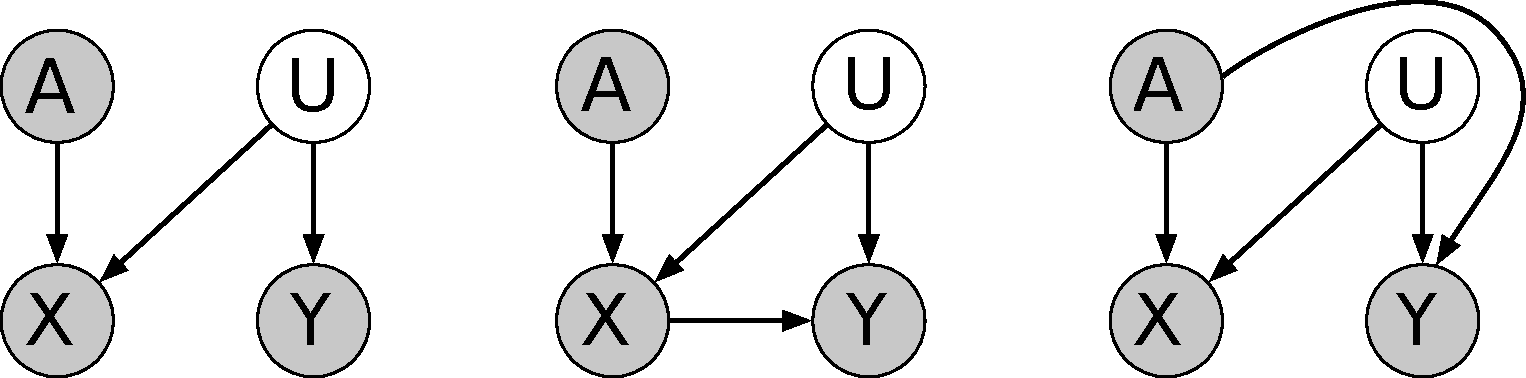
\includegraphics[width=0.9\textwidth]{simple_models_no_q2}}
\vspace{-2ex}
\caption{Three causal models for different real-world fair prediction scenarios.\label{figure.simple_models} See section \ref{sec:count_fair} for discussion.\vspace{-5ex}}
\vspace{-2ex}
\end{center}
\end{figure*}

\subsection{Examples}
To give an intuition for counterfactual fairness we will consider three % real-world
fair prediction scenarios: \textbf{insurance pricing}; \textbf{crime prediction}; \textbf{college admissions}. Each of these correspond to one of the three causal graphs in Figure~\ref{figure.simple_models}, and are discussed below.
%
\paragraph{Scenario 1: The Red Car.}
Imagine a car insurance company wishes to price insurance for car owners by
predicting their accident rate $Y$. They assume there is an
unobserved factor corresponding to aggressive driving $U$, that (a) causes
drivers to be more likely have an accident, and (b) causes individuals to prefer red cars (the observed
variable $X$). Moreover, individuals belonging to a
certain race $A$ are more likely to drive red cars. However, these individuals are no more likely to be aggressive or to get in accidents than any one else. We show this scenario in Figure~\ref{figure.simple_models} (\emph{Left}).

Thus, using the red car feature $X$ to predict accident likelihood $Y$
would seem to be an unfair prediction because it may charge
individuals of a certain race more than others, even though {\em no
  race is more likely to have an accident}. Counterfactual fairness
agrees with this notion.
%
\begin{lem}
  Consider the structure in Figue 2 (Left).  There exist model
classes where fitting a predictor of $Y$ to $X$ only is not counterfactually
fair, while the same algorithm will given a fair predictor using $A$
and $X$.
\end{lem}
%
\begin{proof}
For simplicity, consider the case where the equations described by the model in Figure~\ref{figure.simple_models} (\emph{Left}) are deterministic and linear:
\begin{align}
X = \alpha A + \beta U, \;\;\;\; Y = \gamma U \nonumber
\end{align}
where the coefficients $\alpha,\beta,\gamma$ are given (in practice these are estimated), and by assumption $\alpha \neq 0$. We can test whether the predictor $\hat Y(X)$
defined by least-squares projection of $Y$ on $X$ is counterfactually-fair using the procedure described in Section~\ref{subsec:cmc}:
%\begin{itemize}
{\em (i)} Compute $U$ given observations of $X,A$.%, by solving for $U$. 
{\em (ii)} Substitute the equations involving $A$ with an interventional value $a'$. 
% (i.e., this says: `what happens if the race of an individual were changed')
{\em (iii)} Compute the variables $X,Y$ with the interventional value $a'$.

In this deterministic case we achieve counterfactual fairness only if the predicted value $\hat{Y}(X)$ is identical before and after we change $A$. However, changing $A$ changes $X$. Thus $\hat{Y}(X)$ must be different and the model  is not counterfactually fair.
\end{proof}
The above result holds in a more general case: any non-constant estimator that depends only on a single $X$ is not be counterfactually fair as changing $A$ always alters $X$.
%
%
\paragraph{Scenario 2: High Crime Regions.} 
A local police precinct wants to know how likely a given house is to be broken into, $Y$. This likelihood depends on many unobserved factors
($U$) but also upon the neighborhood the house lies in ($X$). However, different ethnic groups are more likely to live in particular neighborhoods, and so neighborhood and break-in rates are often strongly correlated with the 
race $A$ of the house occupier. This scenario can be seen in Figure~\ref{figure.simple_models} (\emph{Center}). Unlike the previous case, the variable $Y$ itself is not counterfactually fair, so a predictor trained using $X$ and $A$ without additional constraints is unlikely to be fair. 


% In such a scenario, although the likelihood of a particular
% person having their house broken into does not depend upon race
% directly, it does vary which a persons race and so is not
% counterfactually fair.

\paragraph{Scenario 3: University Success.}
A university wants to know if a student is likely to be successful after they graduate $Y$. They have information such as incoming grade point average (GPA), advanced placement (AP) exams results, and other academic features $X$. The university believes however, that an individual's gender may influence these features as well as their post-graduation success $Y$ due to social discrimination. Instead, they would like to model an individual's latent talent $U$ which causes $X$ and $Y$. We show this scenario in Figure~\ref{figure.simple_models} (\emph{Right}).

%  The world on the right shows $Y'$ a
% causally fair variable that doesn't depend on $A$ being directly
% corrupted by a bias relating to $A$, resulting in an observation
% $Y$. In this case, learning a causally fair approximation of $Y$ can
% recover the true variable $Y'$ (up to noise).


% \subsection{Examples}
% To get an intuition for what the different definitions of fairness imply, we will
% revisit the examples of figure \ref{figure.simple_models}.
% begin by describing a few possible real-world scenarios. For each of these we will describe what counterfactually-fair and counterfactually-unfair predictors look like.

% \paragraph{Scenario 1: The Red Car.}
% Imagine a car insurance company wants a quick, anonymous way to determine how to price insurance for different car owners by predicting their accident likelihood $Y$. They've noticed that there is a correlation between driving a red car $X$ and a higher rate of automobile accidents. Thus they would like to increase the insurance for all red car drivers. 

% Imagine what's really going on is shown in Figure~\ref{figure.simple_models} (\emph{Left}). The correlation between have a red car $X$ and accidents $Y$ is due to an `aggressiveness' factor $U$: aggressiveness causes individuals to be in accidents more often, and it also attracts them to red cars. Unfortunately, the red car feature $X$ is also affected by an individual's race $A$. 

% TODO. Here the examples and their motivation can be as follows:

% \begin{itemize}
% \item something analogous to the red car example: $A$ is not a cause of
%   $Y$ but might indirectly bias the result even without using $A$ as a predictor;
% \item something with selection bias, maybe a toy version of COMPAS;
% \item something where an unfair judgment (say, credit score) that can be potentially
%   considered as a target variable, and an
%   ``objective target'' (say, defaulting on a loan) are present, and
%   what the recommendation is
% \end{itemize}
%%% Local Variables:
%%% mode: latex
%%% TeX-master: "ricardo_draft"
%%% End:


\section{Implementing Counterfactual Fairness}
\label{sec:methods}

Varios design choices go in the definition of $\hat Y$ and its fitting. Given a causal model, these choices include the following.

First, $\hat Y$ is a function of $U \cup X$ even if our initial notation emphasizes its dependence on the (possibly random) $U$. This also means it can be a function of a subset of this set, and any element of $X$ which is not a descendant of $A$ can be used. If only a strict subset of $U$ is used, the causal model does not need to be fully specified: equation $V_i = f_i(pa_i, U_{pa_i})$ can be substituted by a non-deterministic conditional probabability $p(V_i\ |\ pa_i, U_{pa_i}')$, where $U_{pa_i}' \subset U_{pa_i}$ and $p(V_i\ |\ pa_i, U_{pa_i}') = \int f_i(pa_i, U_{pa_i}) d U_{pa_i}''$, where $U_{pa_i}'' \equiv U_{pa_i} \backslash U_{pa_i}'$. This marginalization has implications in modeling, as discussed in the next section.

Second, $\hat Y(U)$ is to be understood as a parameterized function $g_\theta(U, X)$ where $\theta$ is learned by minimizing (empirical version of) the expected loss $E[l(Y, g_\theta(U, X))\ | X,
  A]$, where the expectation is over $A \cup X \cup U \cup \{Y\}$. For instance, $l(Y, g_\theta(U, X)) = (Y - g_\theta(U, X))^2$, or the log-loss for Bernoulli classification.  In practice, the distribution of $A \cup X \cup \{Y\}$ can be the empirical distribution as given by some training data, while $p(U\ |\ X, A)$ comes from the estimated causal model fit to the same training data. Markov chain Monte Carlo (MCMC) may be necessary to generate samples from this conditional, which means every training data point is replaced by a set of data points sharing the same $A \cup X \cup \{Y\}$ but with different replicates of $U$. Any predictor can be used as $g_\theta(U, X)$, such as random forests and neural networks.

\subsection{Criticisms, and a User's Guide for Model Building}

Causal modeling requires untestable assumptions. Experimental data can sometimes be used to infer causal connections, but counterfactual modeling adds another layer of complexity by requiring functional decompositions between background and endogenous variables or, equivalently, joint distributions among variables which belong to separate physical realities. Such decompositions are in general not uniquely identifiable even with experimental data, which has motivated causal modeling frameworks that avoid counterfactuals entirely unless where they are strictly necessary \citep{dawid:00}. As in several matters of law and regulation, fairness at an individual level is a counterfactual quantity and some level of counterfactual assumptions are unavoidable. As a guide for building fair predictive models, we categorize assumptions by three levels of increasing strength.

\begin{itemize}
\item[L1] Given a (set of plausible) causal DAG(s), build $\hat Y$
  using as covariates only the observable variables which are not
  descendants of the protected attributes $A$ in the DAG(s).This
  requires (partial) information about the causal DAG, but no
  assumptions about structural equations and priors over background
  variables. Within our definition (\ref{eq:cf_definition}), here
  $\hat Y$ cannot be a function of $U$ but is allowed to be a function
  of any subset of $X$ that is not a descendant of $A$; \item[L2] The above might waste much information, particularly if the
  protected attributes are typical demographic information such as
  race, sex, gender and age, which can be parents but not children of
  other variables in the DAG. To include information from descendants
  of $A$, postulate background latent variables that act as latent
  causes of observable variables, based on explicit domain knowledge
  and learning algorithms with causal assumptions\footnote{In some
    domains, it is actually common to build a model entirely around
    latent constructs which have few or no observable parents nor
    connections among observed variables \citep{bol:89}.}.  As these
  (latent) variables are not descendants of $A$, they can be used.
  Conditioning on descendants of $A$ will propagate information from
  $X$ to them. The dependency of each $V_i$ on its parents can be
  probabilistic, instead of given by a structural equation, as
  explained in the previous section;
\item[L3] In the above construction, the model still factorizes as a
  general DAG model, where each node follows a non-degenerate
  distribution given observed and latent variables. In the final level
  of assumptions, remove all randomness from the conditional
  distributions to obtain a full decomposition $(U, V, F)$ of the
  model. Default assumptions, partially independent of the domain,
  might be invoked. For instance, we can model the conditional
  distribution $p(V_i\ |\ V_1, \dots, V_{i - 1})$ as an additive error
  model, $V_i = f_i(V_1, \dots, V_{i - 1}) + e_i$ \citep{peters:14}. The error
  term $e_i$, now assumed to be a summary of the other latent causes
  of $V_i$, then becomes an input to $\hat Y$ after conditioning on
  the observable variables. This maximizes the amount of information
  that can be properly extracted from a causal model by the fair
  predictor $\hat Y$.
\end{itemize}

A discussion on testing the implications of a given model is beyond the scope of this paper, as there is already a wealth of literature on the topic, with \citep{bollen:93} providing a classic account aimed at structural equation models. There are as well tools that help the (partial) discovery of causal structure \citep{sgs:00,peters:14} and latent variables \citep{silva:10b,HalpernSontag_uai13,anima:14}. The bottom line is that fairness should be the consequence of clear assumptions that need to be defended given the extent of existing available evidence, but with the understanding that there will be a subset of assumptions which cannot be tested. The ultimate validation of a counterfactual model is a matter of agreement between regulators and algorithm designers, lying outside the realm of machine learning theory and within the subject matter of the domain. The goal of counterfactual fairness is to provide a foundation for justifying particular modeling choices, which otherwise may sound arbitrary. With counterfactual fairness, assumptions are laid out in the open for criticism by regulators and society.

\subsection{Special cases}

Consider the graph $A \rightarrow X \rightarrow Y$. In general, if $\hat Y$ is a function of $X$ only, then $\hat Y$ will not obey demographic parity, $p(\hat Y\ |\ A = a) \neq p(\hat Y\ |\ A = a')$.  If we postulate a structural equation $X = \alpha A + e_X$, then given $A$ and $X$ we can deduce $e_X$. If $\hat Y$ is a function of $e_X$ only and if by assumption $e_X$ is independent of $A$, then the assumptions imply that $\hat Y$ will satisfy demographic parity, and that can be falsified.

By way of contrast, if $e_X$ is not uniquely identifiable from the structural equation and $(A, X)$, then the distribution of $\hat Y$ will depend of the value of $A$ as we marginalize $e_X$, and demographic parity will not follow. This leads to the following Lemma:

%\begin{lem}
{\bf Lemma XX} If all background variables $U' \subseteq U$ used in the definition of $\hat Y$ are determined from $(A, W)$, and all observable variables used in the definition of $\hat Y$ are independent of $A$ given $U'$, then $\hat Y$ satisfies demographic parity. If the conditions fail, then $\hat Y$ will not satisfy demographic parity in general. 
%\end{lem}
  
In one sense, definition (\ref{eq:cf_definition}) is a counterfactual demographic parity condition, which is advocated here as a substitute for the more traditional definition.

We also advocate that counterfactual assumptions should underlie all approaches based on separating the sources of variation of the data into ``fair'' and ``unfair'' components. As an example, the method proposed by \cite{louizos2015variational} explains the variability in $X$ from $A$ and an independent source $U$ following the DAG $A \rightarrow X \leftarrow U$. Since $U$ and $A$ are not independent given $X$ in this directed representation, a type of ``posterior regularization'' \citep{ganchev:10} is enforced such that a posterior $p_{fair}(U\ | A, X)$ is close to the model posterior $p(U\ |\ A, X)$ while having the property $p_{fair}(U\ | A = a, X) \approx p_{fair}(U\ | A = a', X)$. But this is neither necessary nor sufficient for counterfactual fairness if the model for $X$ given $A$ and $U$ is not justified by a causal mechanism. If it is, $p(U\ |\ A, X)$ is justified as distribution which we can use to marginalize $U$ in $p(\hat Y(U)\ |\ A, X)$. No posterior regularization is necessary.  Methods which estimate the relationship between $A$, $U$ and $X$ based on penalizing dependence measures between an estimated $U$ and $A$ are relevant in estimating a causal model such as the one described by \citep{mooij:09}, but this is motivated by a model in which $U$ is deterministically inferred from $A$ and $X$ by construction. Moreover, it is unclear in \cite{louizos2015variational} how the ideal label $Y$ is causally connected to $U$ and $A$, so that the semantics of the ``unfair''
components of $Y$ are left unexplained.


\section{Illustration: Law School Success}
\label{sec:experiments}
% !TEX root=ricardo_draft.tex
% In this section we evaluate our framework for modeling fairness.
We illustrate our approach on a practical problem that requires
fairness, the \emph{prediction of success in law school}. A second
problem, \emph{separating actual and perceived criminality in police
  stops}, is described in the Supplementary Material. Following closely the
usual framework for assessing causal models in the machine learning
literature, the goal of this experiment is to quantify how our
algorithm behaves with finite sample sizes while assuming ground truth compatible
with a synthetic model.

\noindent {\bf Problem definition: Law school success}

% From 1991 to 1996
The Law School Admission Council
conducted a survey across 163 law
schools in the United States \cite{wightman1998lsac}. % The survey was
% designed to assess `the law school experience of minority students, as
% well as their ultimate entry into the profession'.
It contains information on 21,790 law students such as their entrance
exam scores (LSAT), their grade-point average (GPA) collected prior to
law school, and their first year average grade (FYA).
%, and following Law
%School i.e. whether students passed the final examination, the `bar
%exam' (P)).

Given this data, a school may wish to predict if an applicant will
have a high FYA.
% from information about their academic performance
% before law school.
The school would also like to make sure these
predictions are not biased by an individual's race and sex. However,
the LSAT, GPA, and FYA scores, may be biased due to social factors. % Our approach will use variables that are
% counterfactually fair for prediction.
We compare our framework with two unfair baselines: 1. \textbf{Full}:
the standard technique of using all features, including sensitive
features such as race and sex to make predictions;
2. \textbf{Unaware}: fairness through unawareness, where we do not use
race and sex as features. For comparison, we generate predictors $\hat
Y$ for all models using logistic regression.


\paragraph{Fair prediction.}
As described in Section~\ref{sec:limit-guide-model}, there are three
ways in which we can model a counterfactually fair predictor of
FYA. Level 1 uses any features which are not descendants of race and
sex for prediction. Level 2 models latent `fair' variables which are
parents of observed variables. These variables are independent of both
race and sex. Level 3 models the data using an additive error model,
and uses the independent error terms to make predictions. These models
make increasingly strong assumptions corresponding to increased
predictive power. We split the dataset 80/20 into a train/test set,
preserving label balance, to evaluate the models.

As we believe LSAT, GPA, and FYA are all biased by race and sex, we
cannot use any observed features to construct a counterfactually fair
predictor as described in Level 1. % Instead we would need to resort to a
% constant predictor% , such as the mean of FYA over the training set
% . % As this model is trivial we do not consider it. 

In Level 2, we postulate that a latent variable: a student's
\textbf{knowledge} (K), affects GPA, LSAT, and FYA scores. The causal
graph corresponding to this model is shown in
Figure~\ref{figure.law_school}, (\textbf{Level 2}). This is a
short-hand for the distributions:
\[
\begin{array}{cc}
  \mbox{GPA} \sim {\cal N}(b_{G} + w_{G}^K K + w_{G}^R R + w_{G}^S S, \sigma_{G}),&  \hspace{0.2in}
  \mbox{FYA} \sim {\cal N}(w_{F}^K K + w_{F}^R R + w_{F}^S S, 1),\\
  \mbox{LSAT} \sim \textrm{Poisson}(\exp(b_{L} + w_{L}^K K + w_{L}^R R + w_{L}^S S)),& \hspace{0.2in}
  \mbox{K} \sim {\cal N}(0,1)
\end{array}
\]
%\begin{align}
%\mbox{GPA} &\sim {\cal N}(b_{G} + w_{G}^K K + w_{G}^R R + w_{G}^S S, \sigma_{G}),
%\mbox{LSAT} &\sim \textrm{Poisson}(\exp(b_{L} + w_{L}^K K + w_{L}^R R + w_{L}^S S)) \nonumber \\
%\mbox{FYA} &\sim {\cal N}(w_{F}^K K + w_{F}^R R + w_{F}^S S, 1), 
%K &\sim {\cal N}(0,1) \nonumber
%\end{align}
% As FYA is already standardized to have mean $0$ and standard
% deviation $1$ we do not learn bias and standard deviation terms.
We perform inference on this model using an observed training set to
estimate the posterior distribution of $K$. We use the probabilistic
programming language Stan \cite{rstan} to learn $K$. We call the
predictor constructed using $K$, \textbf{Fair $K$}.


\begin{figure}[th]
  \hspace{-0.3in}
  \begin{tabular}{p{0.5\columnwidth}p{0.5\columnwidth}}
    \centerline{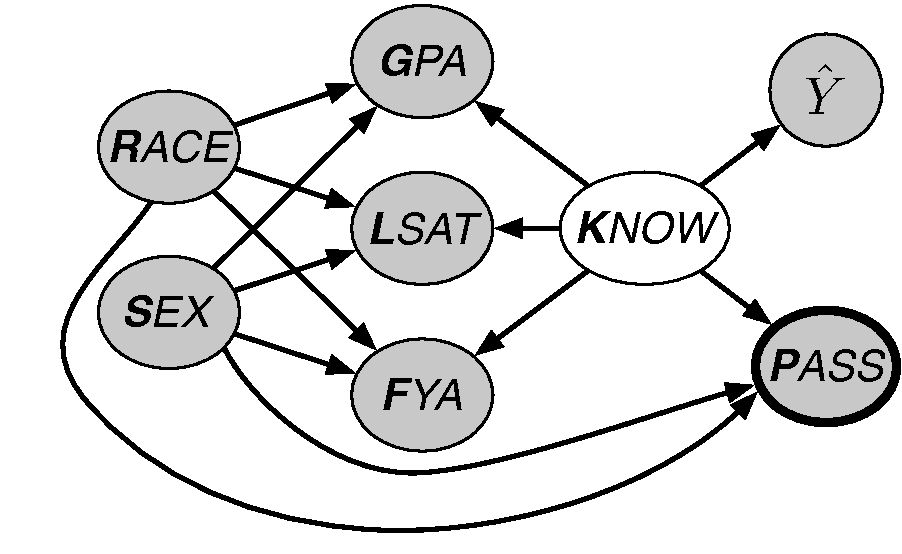
\includegraphics[width=0.4\columnwidth]{law_school_model}}
    &
      \centerline{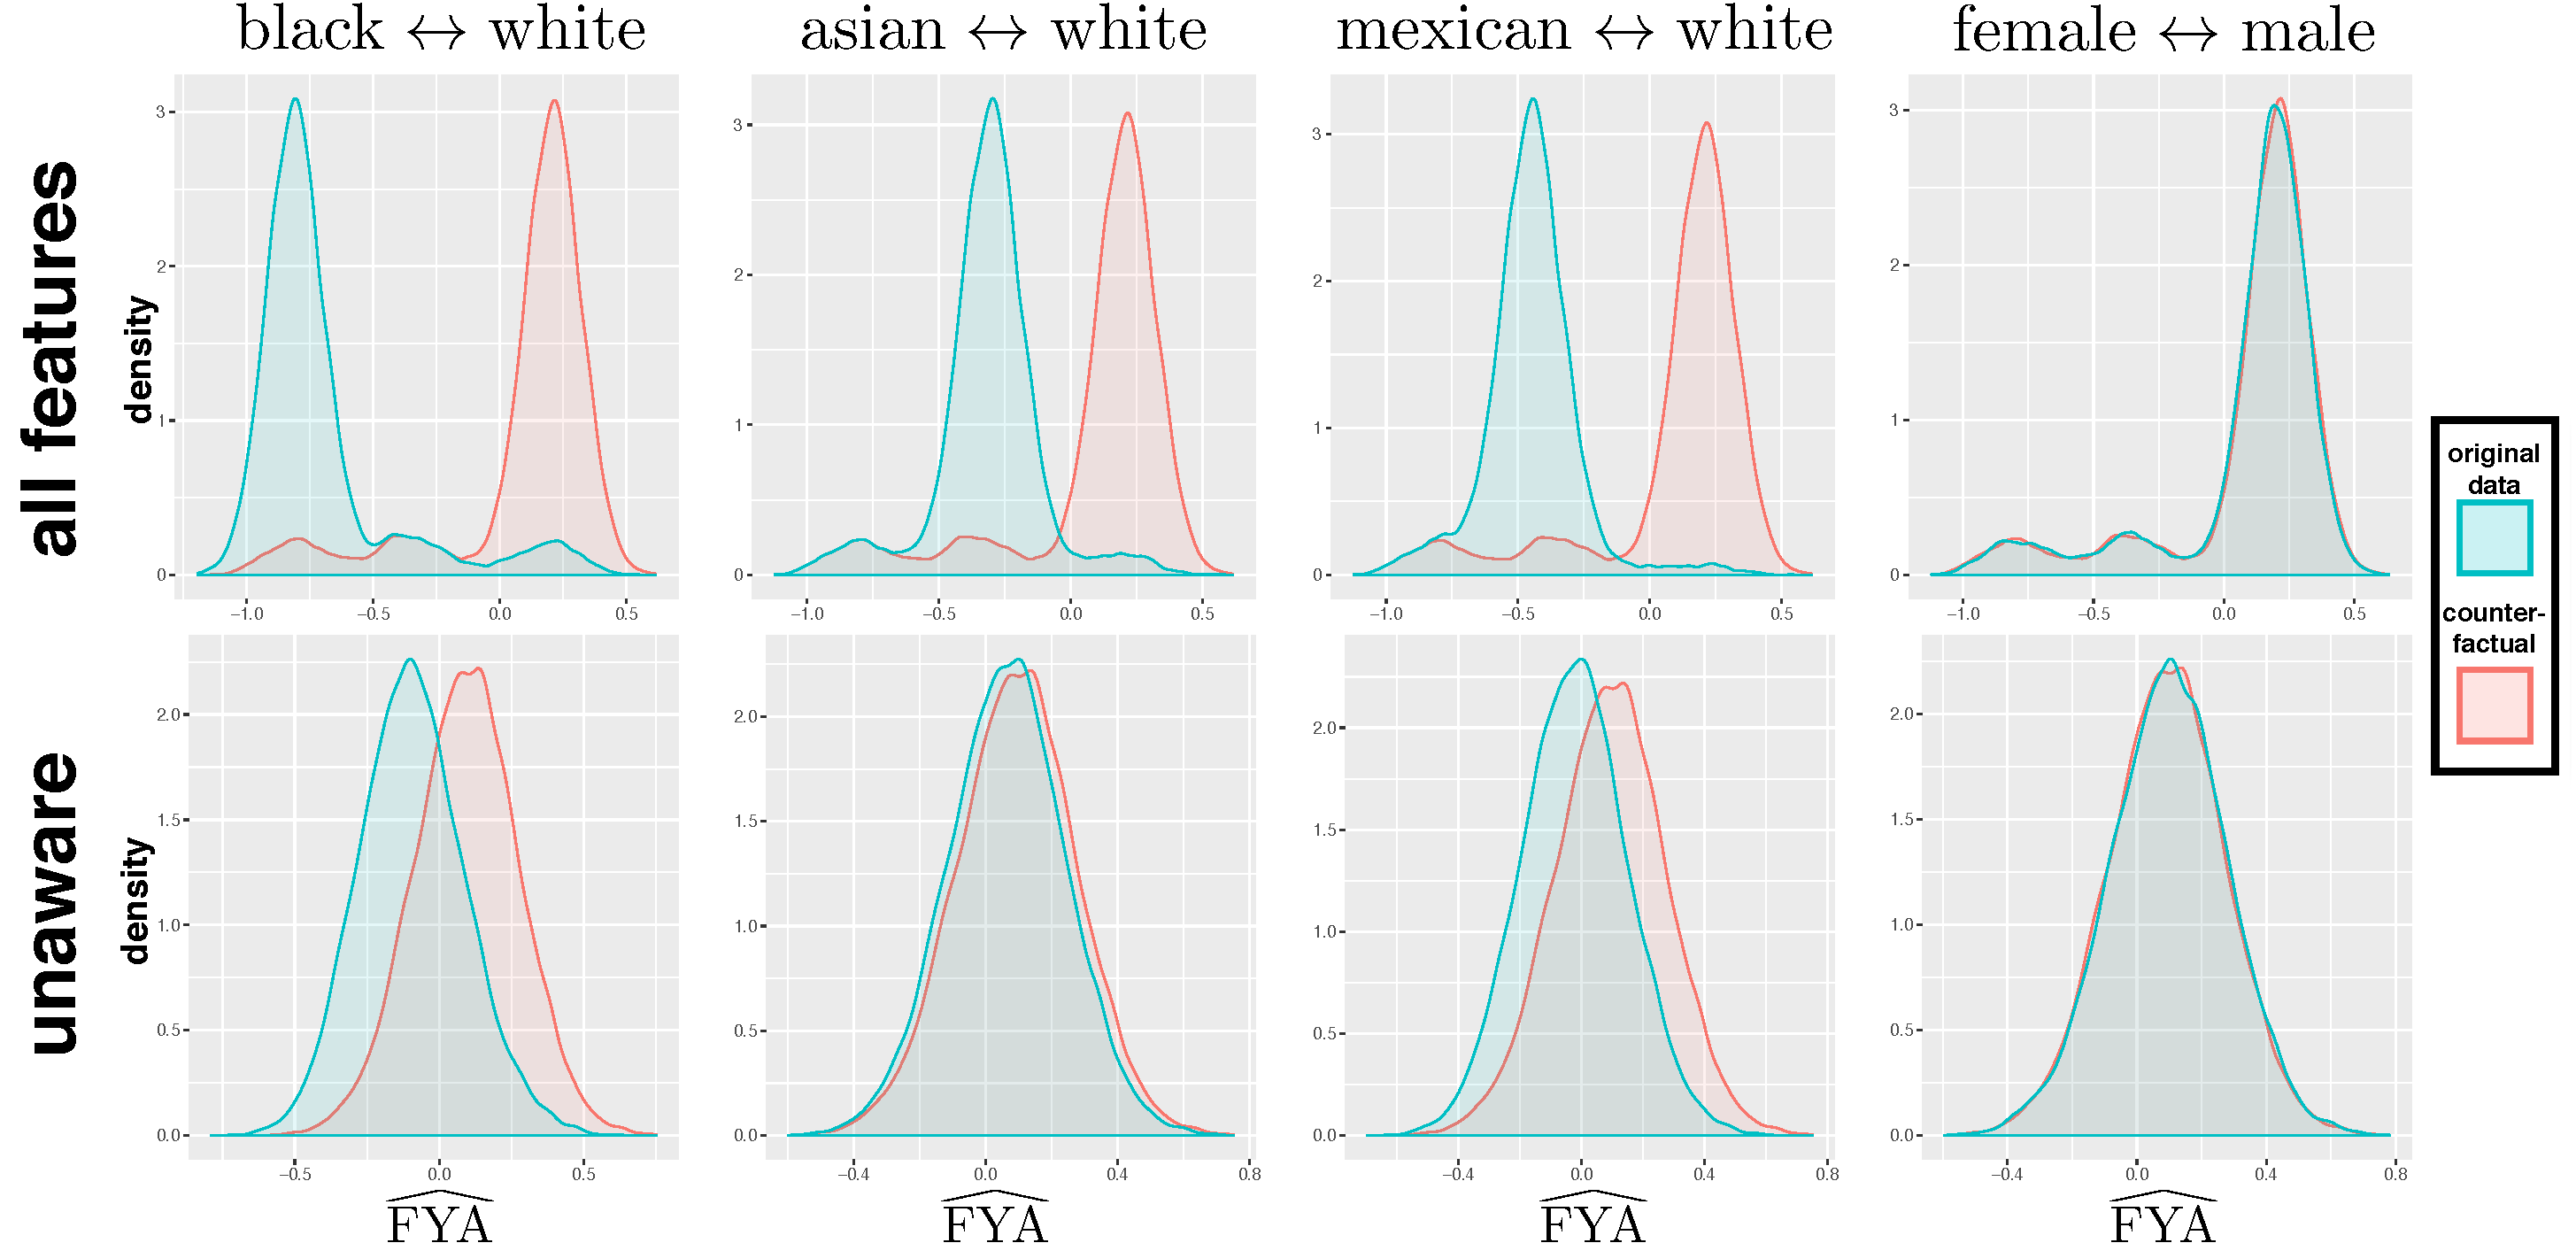
\includegraphics[width=0.5\columnwidth]{counterfactual}}
  \end{tabular}
  \caption{{\bf Left:} A causal model for the problem of predicting law school success fairly.\label{figure.law_school}
  {\bf Right:} Density plots of predicted $\mbox{FYA}_a$ and $\mbox{FYA}_{a'}$.\label{figure.counterfactual}
}
\end{figure}

\begin{table}
\centering
\caption{Prediction results using logistic regression. Note that we
  must sacrifice a small amount of accuracy to ensuring
  counterfactually fair prediction (Fair $K$, Fair Add), versus the
  models that use unfair features: GPA, LSAT, race, sex (Full,
  Unaware).} \label{table.pred_law}
\begin{tabular}{ccccc} 
\hline
 &  {\bf Full} & {\bf Unaware} & {\bf Fair $K$} & {\bf Fair Add} \\
\hline
RMSE & 0.873 & 0.894 & 0.929 & 0.918 \\
%\bf{Method} & %\multicolumn{2}{c}{\bf Full} & \multicolumn{2}{c}{\bf Unaware} & \multicolumn{2}{c}{\bf Fair L2} & \multicolumn{2}{c}{\bf Fair L3} \\
\hline
\end{tabular}
\end{table}

In Level 3, we model GPA, LSAT, and FYA as continuous variables with additive error terms independent of
race and sex (that may in turn be correlated with one-another). This model is shown in
Figure~\ref{figure.law_school}, (\textbf{Level 3}), and is expressed by: % the equations:
\begin{align}
\mbox{GPA} &= b_{G} + w_{G}^R R + w_{G}^S S + \epsilon_G, \;\; \epsilon_G \sim p(\epsilon_G) \nonumber \\
\mbox{LSAT} &= b_{L} + w_{L}^R R + w_{L}^S S + \epsilon_L, \;\; \epsilon_L \sim p(\epsilon_L) \nonumber \\
\mbox{FYA} &= b_{F} + w_{F}^R R + w_{F}^S S + \epsilon_F, \;\; \epsilon_F \sim p(\epsilon_F) \nonumber
\end{align}
We estimate the error terms $\epsilon_G,\epsilon_L$ by first fitting
two models that each use race and sex to individually predict GPA and
LSAT. We then compute the residuals of each model (e.g., $\epsilon_G
\!=\! \mbox{GPA} \!-\! \hat{Y}_{\scriptsize\mbox{GPA}}(R,S)$). We use
these residual estimates of $\epsilon_G,\epsilon_L$ to predict FYA. We
call this \emph{Fair Add}.


% impacts these features.

% We propose to model the law school data as shown in
% Figure~\ref{figure.law_school}. We suspect that variables race and sex
% affect student performance (e.g. GPA, LSAT, and FYA) due to factors
% such as cultural norms, which assume that individuals of a certain
% race or sex are `better suited' to be lawyers. Such beliefs could
% adversely impact students who do not fit these norms. Instead we would
% like to model the latent \emph{knowledge} (K) of a student, which also
% impacts these features. 
% We can then construct a predictor that
% predicts FYA fairly using knowledge. It is easy to show that such a predictor
% is counterfactually fair, whereas a predictor that uses features GPA and
% LSAT is not (in this case even including race and sex as
% features cannot correct this, as can be done in the linear case). The
% causal 
 %; %3. \textbf{Variational Fair Autoencoder (VFAE)} \cite{louizos2015variational}, a recent approach that works to learn a fair representation of the original data.
% compute counterfactuals for both race and sex

\paragraph{Accuracy.}
We compare the RMSE achieved by logistic regression for each of the
models on the test set in Table~\ref{table.pred_law}.  The
\textbf{Full} model achieves the lowest RMSE as it uses race and sex
to more accurately reconstruct FYA. Note that in this case, this model
is not fair even if the data was generated by one of the models shown
in Figure~\ref{figure.law_school} as it corresponds to Scenario 3. The
(also unfair) \textbf{Unaware} model still uses the unfair variables
GPA and LSAT, but because it does not use race and sex it cannot match
the RMSE of the \textbf{Full} model. As our models satisfy
counterfactual fairness, they trade off some accuracy. Our first model
\textbf{Fair $K$} uses weaker assumptions and thus the RMSE is
highest. Using the Level 3 assumptions, as in \textbf{Fair Add} we
produce a counterfactually fair model that trades
slightly stronger assumptions for lower RMSE.


\paragraph{Counterfactual fairness.}
We would like to empirically test whether the baseline methods are
counterfactually fair. To do so we will assume the true model of the
world is given by Figure~\ref{figure.law_school}, (\textbf{Level
  2}). We can fit the parameters of this model using the observed data
and evaluate counterfactual fairness by sampling from
it. Specifically, we will generate samples from the model given either
the observed race and sex, or \emph{counterfactual} race and sex
variables. We will fit models to both the original and counterfactual
sampled data and plot how the distribution of predicted FYA changes
for both baseline models. Figure~\ref{figure.counterfactual} shows
this, where each row corresponds to a baseline predictor and each
column corresponds to the counterfactual change. In each plot, the blue
distribution is density of predicted FYA for the original data and the
red distribution is this density for the counterfactual data. If a
model is counterfactually fair we would expect these distributions to
lie exactly on top of each other. Instead, we note that the
\textbf{Full} model exhibits counterfactual unfairness for all
counterfactuals except sex. We see a similar trend for the
\textbf{Unaware} model, although it is closer to being
counterfactually fair. To see why these models seem to be fair
w.r.t. to sex we can look at weights of the DAG which generates the
counterfactual data. Specifically the DAG weights from (male,female)
to GPA are ($0.93$,$1.06$) and from (male,female) to LSAT are
($1.1$,$1.1$). Thus, these models are fair w.r.t. to sex simply
because of a very weak causal link between sex and GPA/LSAT.

% here describe what we see

% maybe sample from model and check it out
%\paragraph{Model validity.}
 

% TODO rank top 10 students by ability or by other score in law_school.py which only considers observed features


% \begin{table}[t]
% \vspace{-2ex}
% \caption{}
% \vspace{-3ex}
% \label{table.pred_law}
% \begin{center}
% \resizebox{\columnwidth}{!}
% {
% \begin{sc}
% \footnotesize
% \begin{tabular}{c|c|c|c}
% \hline
% %\multicolumn{5}{c}{\textbf{Lower Bounds}}\\
% \hline
% & full & unaware  & fair l2 & fair l3 \\
% \hline
% RMSE & 0.873 & 0.894 & 0.929 & 0.918 \\ \hline
% \end{tabular}
% \end{sc}
% }
% \end{center}
% \vspace{-4ex}
% \end{table}

%{lr@{$\pm$}lr@{$\pm$}lr@{$\pm$}l}

%\subsection{Model criticism}
%%% Local Variables:
%%% mode: latex
%%% TeX-master: "ricardo_draft"
%%% End:


\section{Conclusion}
\label{sec:conclusion}
We have presented a new model of fairness we refer to as {\em
  counterfactual fairness}. It allows us to propose algorithms
that, rather than simply ignoring protected attributes, are able to
take into account the different social biases that may arise towards
individuals based on ethically sensitive attributes
and compensate
for these biases effectively. We experimentally contrasted our
approach with previous fairness approaches and show that our explicit
causal models capture these social biases and make clear the implicit
trade-off between prediction accuracy and fairness in an unfair
world. We propose that fairness should be regulated by explicitly
modeling the causal structure of the world. Criteria based purely on
probabilistic independence cannot satisfy this and are unable to
address \emph{how} unfairness is occurring in the task at hand. By
providing such causal tools for addressing fairness questions we hope
we can provide practitioners with customized techniques for solving a
wide array of fairness modeling problems.

\bibliography{rbas,bibliography}
\bibliographystyle{icml2017}

\newpage
% !TEX root=ricardo_draft.tex
% In this section we evaluate our framework for modeling fairness.

%%%% TODO!!! ADD COMMENT THAT WE NEED Y TO LEARN THE CAUSAL MODEL!!!!!

\section*{S1 Population Level vs Individual Level Causal Effects}
\label{sec:individual}

As discussed in Section~\ref{sec:count_fair}, counterfactual fairness
is an individual-level definition. This is fundamentally different
from comparing different units that happen to share the same
“treatment” $A = a$ and coincide on the values of $X$. To see in
detail what this means, consider the following thought experiment.

Let us assess the causal effect of $A$ on $\hat Y$ by controlling
$A$ at two levels, $a$ and $a'$. In Pearl's notation, where ``$do(A = a)$''
expresses an intervention on $A$ at level $a$, we have that
\begin{equation}
\label{eq:ace}
\mathbb{E}[\hat Y\ |\ do(A = a), X = x] - \mathbb{E}[\hat Y\ |\ do(A = a'), X = x],
\end{equation}
is a measure of causal effect, sometimes called the average causal
effect (ACE). It expresses the change that is expected when we
intervene on $A$ while observing the attribute set $X = x$, under two
levels of treatment. If this effect is non-zero, $A$ is considered to
be a cause of $\hat Y$.

This raises a subtlety that needs to be addressed: in general, this
effect will be non-zero {\it even if $\hat Y$ is counterfactually
  fair}. This may sound counter-intuitive: protected attributes such
as race and gender are causes of our counterfactually fair decisions.

In fact, this is not a contradiction, as the ACE in Equation
(\ref{eq:ace}) is different from counterfactual effects. The ACE
contrasts two independent exchangeable units of the population, and it
is a perfectly valid way of performing decision analysis. However, the
value of $X = x$ is affected by different background variables
corresponding to different individuals. That is, the causal effect
(\ref{eq:ace}) contrasts two units that receive different treatments
but which happen to coincide on $X = x$. To give a synthetic example,
imagine the simple structural equation
\[
X = A + U.
\]

The ACE quantifies what happens among people with $U = x -
a$ against people with $U' = x - a'$. If, for instance, $\hat Y =
\lambda U$ for $\lambda \neq 0$, then the effect \eqref{eq:ace}
is $\lambda(a - a') \neq 0$.

Contrary to that, the counterfactual difference is zero.
That is,
\[
\mathbb{E}[\hat Y_{A \leftarrow a}(U)\ |\ A = a, X = x] -
\mathbb{E}[\hat Y_{A \leftarrow a'}(U)\ |\ A = a, X = x] =
\lambda U - \lambda U = 0.
\]

In another perspective, we can interpret the above just as if we had
{\it measured} $U$ from the beginning rather than performing
abduction. We then generate $\hat Y$ from some $g(U)$, so $U$ is the
within-unit cause of $\hat Y$ and not $A$.

If $U$ cannot be deterministically derived from $\{A = a, X = x\}$,
the reasoning is similar. By abduction, the distribution of $U$ will
typically depend on $A$, and hence so will $\hat Y$ when marginalizing
over $U$. Again, this seems to disagree with the intuition that our
predictor should be not be caused by $A$. However, this once again is
a comparison {\it across individuals}, not within an individual. 

It is this balance among $(A, X, U)$ that explains, in the examples
of Section~\ref{sec:further_examples}, why some predictors are
counterfactually fair even though they are functions of the same
variables $\{A, X\}$ used by unfair predictors: such functions must
correspond to particular ways of balancing the observables that, by
way of the causal assumptions, cancel out the effect of $A$.

\noindent {\bf More on conditioning and alternative definitions.} As discussed in
Example 4.4.4 of \citet{pearl:16}, a different proposal for
assessing fairness can be defined via the following concept:
\begin{define}[Probability of sufficiency]
  We define the probability of event $\{ A = a \}$ being a
  \emph{sufficient cause} for our
  decision $\hat Y$, contrasted against $\{ A = a' \}$, as
\begin{align}
  P(\hat Y_{A \leftarrow a'\ }(U) \neq y\ |\ X = x, A = a, \hat Y = y).
  \label{eq:sufficiency}
\end{align}
\end{define}

We can then, for instance, claim that $\hat Y$ is a fair predictor if
this probability is below some pre-specified bound for all $(x, a,
a')$. The shortcomings of this definition come from its original
motivation: to {\it explain} the behavior of an {\it existing}
decision protocol, where $\hat Y$ is the current practice and which in a
unclear way is conflated with $Y$. The implication is that if $\hat Y$
is to be designed instead of being a natural measure of existing
behaviour, then we are using $\hat Y$ itself as evidence for the
background variables $U$. This does not make sense if $\hat Y$ is
yet to be designed by us. If $\hat Y$ is to be interpreted as $Y$, then this
does not provide a clear recipe on how to build $\hat Y$: while we can
use $Y$ to learn a causal model, we cannot use it to collect training
data evidence for $U$ {\it as the outcome $Y$ will not be available to
  us at prediction time}. For this reason, we claim that while
probability of sufficiency is useful as a way of assessing an existing
decision making process, it is not as natural as counterfactual
fairness in the context of machine learning.

\noindent {\bf Approximate fairness and model validation.} The notion
of probability of sufficiency raises the question on how to define
approximate, or high probability, counterfactual fairness. This is an
important question that we address in \citep{russell:17}. Before
defining an approximation, it is important to first expose in detail
what the exact definition is, which is the goal of this paper.

We also do not address the validation of the causal assumptions used
by the input causal model of the {\sc FairLearning} algorithm in
Section \ref{sec:algorithm}. The reason is straightforward: this
validation is an entirely self-contained step of the implementation of
counterfactual fairness. An extensive literature already exists in
this topic which the practitioner can refer to (a classic account for
instance is \cite{bollen:93}), and which can be used as-is in our
context.

The experiments performed in Section \ref{sec:experiments} can be
criticized by the fact that they rely on a model that obeys our
assumptions, and ``obviously'' our approach should work better than
alternatives. This criticism is not warranted: in machine learning,
causal inference is typically assessed through simulations which
assume that the true model lies in the family covered by the
algorithm.  Algorithms, including {\sc FairLearning}, are justified in
the population sense. How different competitors behave with finite
sample sizes is the primary question to be studied in an empirical
study of a new concept, where we control for the correctness of the
assumptions. Although sensitivity analysis is important, there are
many degrees of freedom on how this can be done. Robustness issues are
better addressed by extensions focusing on approximate versions of 
counterfactual fairness. This will be covered in later work.

\noindent {\bf Stricter version.} For completeness of exposition,
notice that the definition of counterfactual fairness could be
strengthened to
\begin{align}
  \label{eq:stricter}
  P(\{\hat Y_{A \leftarrow a}(U) = \hat Y_{A \leftarrow a'}(U)\} = 1\ |\ X = x, A = a).
\end{align}

\noindent This is different from the original definition in the case
where $\hat Y(U)$ is a random variable with a different source of
randomness for different counterfactuals (for instance, if $\hat Y$ is
given by some black-box function of $U$ with added noise that is
independent across each countefactual value of $A$). In such a
situation, the event $\{\hat Y_{A \leftarrow a}(U) = \hat Y_{A
  \leftarrow a'}(U)\}$ will itself have probability zero even if
$P(\hat Y_{A \leftarrow a}(U) = y\ |\ X = x, A = a) = P(\hat Y_{A
  \leftarrow a'}(U) = y\ |\ X = x, A = a)$ for all $y$. We do not
consider version (\ref{eq:stricter}) as in our view it does not feel
as elegant as the original, and it is also unclear whether adding an
independent source of randomness fed to $\hat Y$ would itself be
considered unfair. Moreover, if $\hat Y(U)$ is assumed to be a
deterministic function of $U$ and $X$, as in {\sc FairLearning}, then
the two definitions are the same\footnote{Notice that $\hat Y(U)$ is
  itself a random variable if $U$ is, but the source of randomness,
  $U$, is the same across all counterfactuals.}. Informally, this
stricter definition corresponds to a notion of ``almost surely
equality'' as opposed to ``equality in distribution.'' Without
assuming that $\hat Y$ is a deterministic function of $U$ and $X$,
even the stricter version does not protect us against measure zero events
where the counterfactuals are different. The definition of
counterfactual fairness concisely emphasizes that $U$ can be a random
variable, and clarifies which conditional distribution it follows. Hence, it is our
preferred way of introducing the concept even though it does not
explicit suggests whether $\hat Y(U)$ has random inputs besides $U$.

\section*{S2 Relation to Demographic Parity}
%
Consider the graph $A \rightarrow X \rightarrow Y$. In general, if
$\hat Y$ is a function of $X$ only, then $\hat Y$ need not obey
demographic parity, i.e.
\begin{align}
  P(\hat Y\ |\ A = a) \neq P(\hat Y\ |\ A = a'),\nonumber
\end{align}
\noindent where, since $\hat Y$ is a function of $X$, the
probabilities are obtained by marginalizing over $P(X\ |\ A = a)$ and
$P(X\ |\ A = a')$, respectively.

If we postulate a structural equation $X = \alpha A + e_X$, then given
$A$ and $X$ we can deduce $e_X$. If $\hat Y$ is a function of $e_X$
only and, by assumption, $e_X$ is marginally independent of $A$, then
$\hat Y$ is marginally independent of $A$: this follows the
interpretation given in the previous section, where we interpret $e_X$
as ``known'' despite being mathematically deduced from the
observation $(A = a, X = x)$. Therefore, the assumptions imply that
$\hat Y$ will satisfy demographic parity, and that can be falsified.
By way of contrast, if $e_X$ is not uniquely identifiable from the
structural equation and $(A, X)$, then the distribution of $\hat Y$
depends on the value of $A$ as we marginalize $e_X$, and demographic
parity will not follow. This leads to the following:
%
\begin{lem}
If all background variables $U' \subseteq U$ in the definition of
$\hat Y$ are determined from $A$ and $X$,
and all observable variables in the definition of $\hat Y$ are
independent of $A$ given $U'$, then $\hat Y$ satisfies demographic
parity.
% If the conditions fail, then $\hat Y$ will not satisfy demographic parity in general. 
\end{lem}
Thus, counterfactual fairness can be thought of as a counterfactual
analog of demographic parity, as present in the Red Car example further discussed
in the next section.

\section*{S3 Examples Revisited}

In Section \ref{sec:further_examples}, we discussed two examples. We
reintroduce them here briefly, add a third example, and explain some
consequences of their causal structure to the design of
counterfactually fair predictors.

\paragraph{Scenario 1: The Red Car Revisited.}
In that scenario, the structure $A \rightarrow X \leftarrow U
\rightarrow Y$ implies that $\hat Y$ should not use either $X$ or
$A$. On the other hand, it is acceptable to use $U$.  It is
interesting to realize, however, that since $U$ is related to $A$ and
$X$, there will be some association between $Y$ and $\{A, X\}$ as
discussed in Section S1. In particular, if the structural equation for
$X$ is linear, then $U$ is a linear function of $A$ and $X$, and as
such $\hat Y$ will also be a function of both $A$ and $X$. This is not
a problem, as it is still the case that the model implies that this is
merely a functional dependence that disappears by conditioning on a
postulated latent attribute $U$. Surprisingly, we must make $\hat Y$ a
indirect function of $A$ if we want a counterfactually fair predictor,
as shown in the following Lemma.

  %
\begin{lem}
Consider a linear model with the structure in
Figure~\ref{figure.simple_models}(a).  Fitting a linear predictor to
$X$ \emph{only} is not counterfactually fair, while the same algorithm
will produce a fair predictor using \emph{both} $A$ and $X$.
\end{lem}

\begin{proof}
As in the definition, we will consider the population case, where the
joint distribution is known. Consider the case where the equations
described by the model in Figure~\ref{figure.simple_models}(a)
are deterministic and linear:
\begin{align}
X = \alpha A + \beta U, \;\;\;\; Y = \gamma U. \nonumber
\end{align}
Denote the variance of $U$ as $v_U$, the variance of $A$ as $v_A$, and
assume all coefficients are non-zero. The predictor $\hat Y(X)$
defined by least-squares regression of $Y$ on \emph{only} $X$ is given
by $\hat Y(X) \equiv \lambda X$, where $\lambda = Cov(X, Y) / Var(X)
\!=\! \beta\gamma v_U / (\alpha^2 v_A + \beta^2 v_U) \neq 0$. This 
predictor follows the concept of fairness through unawareness.

We can test whether a predictor $\hat{Y}$ is counterfactually fair
by using the procedure described in Section~\ref{subsec:cmc}:

%\begin{itemize}
{\em (i)} Compute $U$ given observations of $X,Y,A$; %, by solving for $U$.
{\em (ii)} Substitute the equations involving $A$ with an interventional value $a'$; 
% (i.e., this says: `what happens if the race of an individual were changed')
{\em (iii)} Compute the variables $X,Y$ with the interventional value
$a'$. It is clear here that $\hat Y_a(U) \!=\! \lambda(\alpha a +
\beta U) \neq \hat Y_{a'}(U)$. This predictor is not counterfactually
fair. Thus, in this case fairness through unawareness actually
perpetuates unfairness.

Consider instead doing least-squares regression of $Y$ on $X$
\emph{and} $A$. Note that $\hat Y(X,A) \equiv \lambda_X X + \lambda_A
A$ where $\lambda_X,\lambda_A$ can be derived as follows:

\begin{align}
\begin{pmatrix}
\lambda_X \\
\lambda_A
\end{pmatrix} &=
\begin{pmatrix}
Var(X) & Cov(A,X) \\
Cov(X,A) & Var(A)
\end{pmatrix}^{-1}
\begin{pmatrix}
Cov(X,Y) \\
Cov(A,Y)
\end{pmatrix} \nonumber \\
&=
%\frac{1}{(\alpha^2 v_A + \beta^2 v_U)v_A - \alpha^2 v_A^2}
\frac{1}{\beta^2 v_U v_A}
\begin{pmatrix}
v_A & -\alpha v_A \\
-\alpha v_A & \alpha^2 v_A + \beta^2 v_U
\end{pmatrix}
\begin{pmatrix}
\beta \gamma v_U \\
0
\end{pmatrix} \nonumber \\
&=
\begin{pmatrix}
\frac{\gamma}{\beta} \\
\frac{-\alpha\gamma}{\beta}
%(-\alpha\gamma) / \beta
\end{pmatrix}
\end{align}
Now imagine we have observed $A\!=\!a$. This implies that $X = \alpha
a + \beta U$ and our predictor is $\hat Y(X,a) =
\frac{\gamma}{\beta}(\alpha a + \beta U) + \frac{-\alpha\gamma}{\beta}
a = \gamma U$. Thus, if we substitute $a$ with a counterfactual $a'$
(the action step described in Section~\ref{subsec:cmc}) the predictor
$\hat Y(X,A)$ is unchanged. This is because our predictor is
constructed in such a way that any change in $X$ caused by a change in
$A$ is cancelled out by the $\lambda_A$. Thus this predictor is
counterfactually fair.
% This is known to be equivalent to first getting the residuals $R_X$ of $X$ regressed on $A$
% and regressing $Y$ on $R_X$ and $A$. Notice that $R_X \!=\! U$, and $A$ is independent of $U$
% and $Y$. Hence, $\hat Y$ will be the least squares regression of
% $Y$ on $U$, resulting on $\hat Y \!=\! \gamma U$, which is counterfactually fair.
\end{proof}

Note that if Figure~\ref{figure.simple_models}(a) is the
true model for the real world then $\hat Y(X,A)$ will also satisfy
demographic parity and equality of opportunity as $\hat Y$ will be
unaffected by $A$. 

The above lemma holds in a more general case for the structure given
in Figure~\ref{figure.simple_models}(a): any non-constant
estimator that depends only on $X$ is not counterfactually fair as
changing $A$ always alters $X$.
%We also point out that the method
%used in the proof is a special case of a general method to building a
%predictor based on information deduced about $U$ that will be
%described in the next section.

\paragraph{Scenario 2: High Crime Regions Revisited.}

The causal structure differs from the previous example by the extra
edge $X \rightarrow Y$. For illustration purposes, assume again that
the model is linear. Unlike the previous case, a predictor $\hat Y$
trained using $X$ and $A$ is not counterfactually fair. The only
change from Scenario 1 is that now $Y$ depends on $X$ as follows: $Y
\!=\! \gamma U + \theta X$. Now if we solve for $\lambda_X,\lambda_A$
it can be shown that $\hat Y(X,a) \!=\! (\gamma - \frac{\alpha^2
  \theta v_A}{\beta v_U})U + \alpha \theta a$. As this predictor
depends on the values of $A$ that are not explained by $U$, then
$\hat Y(X,a) \!\neq\! \hat Y(X,a')$ and thus $\hat Y(X,A)$ is not
counterfactually fair.

The following extra example complements the previous two examples.

\paragraph{Scenario 3: University Success.}
A university wants to know if students will be successful
post-graduation $Y$. They have information such as: grade point
average (GPA), advanced placement (AP) exams results, and other
academic features $X$. The university believes however, that an
individual's gender $A$ may influence these features and their
post-graduation success $Y$ due to social discrimination. They also
believe that independently, an individual's latent talent $U$ causes
$X$ and $Y$. The structure is similar to
Figure~\ref{figure.simple_models}(a), with the extra
edge $A \rightarrow Y$. We can again ask, is the predictor $\hat
Y(X,A)$ counterfactually fair? In this case, the different between
this and Scenario 1 is that $Y$ is a function of $U$ and $A$ as
follows: $Y \!=\! \gamma U + \eta A$. We can again solve for
$\lambda_X,\lambda_A$ and show that $\hat Y(X,a) \!=\! (\gamma -
\frac{\alpha \eta v_A}{\beta v_U})U + \eta a$. Again $\hat Y(X,A)$ is
a function of $A$ not explained by $U$, so it cannot be counterfactually fair.

% We propose to model the law school data as shown in
% Figure~\ref{figure.law_school}. We suspect that variables race and sex
% affect student performance (e.g. GPA, LSAT, and FYA) due to factors
% such as cultural norms, which assume that individuals of a certain
% race or sex are `better suited' to be lawyers. Such beliefs could
% adversely impact students who do not fit these norms. Instead we would
% like to model the latent \emph{knowledge} (K) of a student, which also
% impacts these features. 
% We can then construct a predictor that
% predicts FYA fairly using knowledge. It is easy to show that such a predictor
% is counterfactually fair, whereas a predictor that uses features GPA and
% LSAT is not (in this case even including race and sex as
% features cannot correct this, as can be done in the linear case). The
% causal 
 %; %3. \textbf{Variational Fair Autoencoder (VFAE)} \cite{louizos2015variational}, a recent approach that works to learn a fair representation of the original data.
% compute counterfactuals for both race and sex

% \begin{table}[t]
% \vspace{-2ex}
% \caption{}
% \vspace{-3ex}
% \label{table.pred_law}
% \begin{center}
% \resizebox{\columnwidth}{!}
% {
% \begin{sc}
% \footnotesize
% \begin{tabular}{c|c|c|c}
% \hline
% %\multicolumn{5}{c}{\textbf{Lower Bounds}}\\
% \hline
% & full & unaware  & fair l2 & fair l3 \\
% \hline
% RMSE & 0.873 & 0.894 & 0.929 & 0.918 \\ \hline
% \end{tabular}
% \end{sc}
% }
% \end{center}
% \vspace{-4ex}
% \end{table}
%
%{lr@{$\pm$}lr@{$\pm$}lr@{$\pm$}l}

\section*{S4 Analysis of Individual Pathways}
\label{sec:pathways}

By way of an example, consider the following adaptation of the
scenario concerning claims of gender bias in UC Berkeley's admission
process in the 1970s, commonly used a textbook example of Simpson's
Paradox. For each candidate student's application, we have $A$ as a
binary indicator of whether the applicant is female, $X$ as the choice
of course to apply for, and $Y$ a binary indicator of whether the
application was successful or not.  Let us postulate the causal graph
that includes the edges $A \rightarrow X$ and $X \rightarrow Y$ only.
We observe that $A$ and $Y$ are negatively associated, which in first
instance might suggest discrimination, as gender is commonly accepted
here as a protected attribute for college admission. However, in the
postulated model it turns out that $A$ and $Y$ are causally independent given
$X$. More specifically, women tend to choose more competitive courses
(those with higher rejection rate) than men when applying.  Our
judgement is that the higher rejection among female than male
applicants is acceptable, if the mechanism $A \rightarrow X$ is
interpreted as a choice which is under the control of the applicant.
That is, free-will overrides whatever possible cultural background conditions
that led to this discrepancy. In the framework of counterfactual
fairness, we could claim that $A$ is not a protected attribute to
begin with once we understand how the world works, and that including
$A$ in the predictor of success is irrelevant anyway once we include
$X$ in the classifier.

However, consider the situation where there is an edge $A \rightarrow
Y$, interpreted purely as the effect of discrimination after causally
controlling for $X$.  While it is now reasonable to postulate $A$ to
be a protected attribute, we can still judge that $X$ is not an unfair
outcome: there is no need to ``deconvolve'' $A$ out of $X$ to obtain
an estimate of the other causes $U_X$ in the $A \rightarrow X$
mechanism. This suggests a simple modification of the definition of
counterfactual fairness. First, given the causal graph $\mathcal G$ assumed to
encode the causal relationships in our system, define $\mathcal P_{\mathcal G_A}$ as
the set of all directed paths from $A$ to $Y$ in $\mathcal G$ which
are postulated to correspond to all unfair chains of events where $A$
causes $Y$. Let $X_{\mathcal P^c_{\mathcal G_A}} \subseteq X$ be the
subset of covariates not present in any path in $\mathcal P_{\mathcal
  G_A}$. Also, for any vector $x$, let $x_s$ represent the
corresponding subvector indexed by $S$. The corresponding uppercase
version $X_S$ is used for random vectors.

\begin{define}[(Path-dependent) counterfactual fairness]
  Predictor $\hat Y$ is {\bf (path-dependent) counterfactually fair}
  with respect to path set $\mathcal P_{\mathcal G_A}$ if under any
  context $X = x$ and $A = a$,
  \label{eq:cf_definition}
\begin{align}
  P(\hat Y_{A \leftarrow a, X_{\mathcal P^c_{\mathcal G_A}} \leftarrow\ x_{\mathcal P^c_{\mathcal G_A}}}(U) = y\ |\ X = x, A = a)  =
  \nonumber\\ 
  P(\hat Y_{A \leftarrow a', X_{\not \mathcal P^c_{\mathcal G_A}} \leftarrow\ x_{ \mathcal P^c_{\mathcal G_A}}}(U) = y\ |\ X = x, A = a), 
\end{align}
for all $y$ and for any value $a'$ attainable by $A$.
\end{define}

This notion is related to {\it controlled direct effects}
\citep{pearl:16}, where we intervene on some paths from $A$ to $Y$,
but not others. Paths in $\mathcal P_{\mathcal G_A}$ are considered
here to be the ``direct'' paths, and we condition on $X$ and $A$
similarly to the definition of probability of sufficiency
(\ref{eq:sufficiency}). This definition is the same as the original
counterfactual fairness definition for the case where $\mathcal
P^c_{\mathcal G_A} = \emptyset$. Its interpretation is analogous to
the original, indicating that for any $X_0 \in X_{\mathcal
  P^c_{\mathcal G_A}}$ we are allowed to propagate information from
the factual assigment $A = a$, along with what we learned about the
background causes $U_{X_0}$, in order to reconstruct $X_0$. The
contribution of $A$ is considered acceptable in this case and does not
need to be ``deconvolved.''  The implication is that any member of
$X_{\not \mathcal P^c_{\mathcal G_A}}$ can be included in the
definition of $\hat Y$. In the example of college applications, we are
allowed to use the choice of course $X$ even though $A$ is a
confounder for $X$ and $Y$. We are still not allowed to use $A$
directly, bypassing the background variables.

As discussed by \cite{nabi:17}, there are some counterfactual
manipulations useable in a causal definition of fairness that can be
performed by exploiting only independence constraints among the
counterfactuals: that is, without requiring the explicit description
of structural equations or other models for latent variables. A
contrast between the two approaches is left for future work, although
we stress that they are in some sense complementary: we are motivated
mostly by problems such as the one in Figure \ref{fig:ex1}(d), where
many of the mediators themselves are considered to be unfairly
affected by the protected attribute, and independence constraints
among counterfactuals alone are less likely to be useful in
identifying constraints for the fitting of a fair predictor.

\begin{figure}[th]
\begin{center}
\centerline{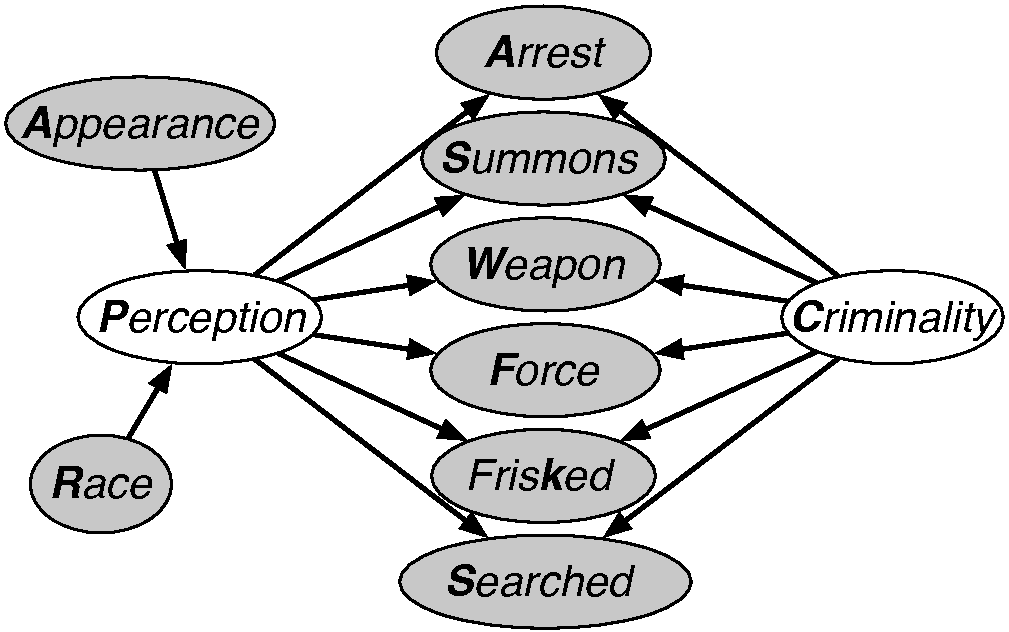
\includegraphics[width=3in]{stop_and_frisk_model3.pdf}}
\caption{A causal model for the stop and frisk dataset.\label{figure.stop_and_frisk}}
\end{center}
\end{figure}

\section*{S5 The Multifaceted Dynamics of Fairness}
\label{sec:dynamics}

One particularly interesting question was raised by one of the
reviewers: what is the effect of continuing discrimination after fair
decisions are made?  For instance, consider the case where banks
enforce a fair allocation of loans for business owners regardless of,
say, gender. This does not mean such businesses will thrive at a
balanced rate if customers continue to avoid female owned business at
a disproportionate rate for unfair reasons. Is there anything useful
that can be said about this issue from a causal perspective?

The work here proposed regards only what we can influence by changing
how machine learning-aided decision making takes place at specific
problems. It cannot change directly how society as a whole carry on
with their biases. Ironically, it may sound unfair to banks to enforce
the allocation of resources to businesses at a rate that does not
correspond to the probability of their respective success, even if the
owners of the corresponding businesses are not to be blamed by
that. One way of conciliating the different perspectives is by
modeling how a fair allocation of loans, even if it does not come
without a cost, can nevertheless increase the proportion of successful
female businesses compared to the current baseline. This change can by
itself have an indirect effect on the culture and behavior of a
society, leading to diminishing continuing discrimination by a
feedback mechanism, as in affirmative action. We believe that in the
long run isolated acts of fairness are benefitial even if we do not
have direct control on all sources of unfairness in any specific
problem.  Causal modeling can help on creating arguments about the
long run impact of individual contributions as e.g. a type of
macroeconomic assessment. There are many challenges, and we should not
pretend that precise answers can be obtained, but in theory we should
aim at educated quantitative assessments validating how a systemic
improvement in society can emerge from localized ways of addressing
fairness.

\section*{S6 Case Study: Criminality vs. Perceived Criminality}
\label{sec:true-vs.-perceived}

We test our approach on a problem of \emph{separating actual and
  perceived criminality in police stops}. For this problem, we
construct a causal model, and make explicit how unfairness may affect
observed and unobserved variables in the world. Given the model we
derive counterfactually fair predictors, and predict latent variables
such as a person's `criminality' (which may be useful for predicting
crime) as well as their `perceived criminality' (which may be due to
prejudices based on appearance). Finally we judge how well our
counterfactually fair `criminality' score satisfies demographic
parity.

\begin{figure}[!th]
\begin{center}
%\vspace{-1ex}
\centerline{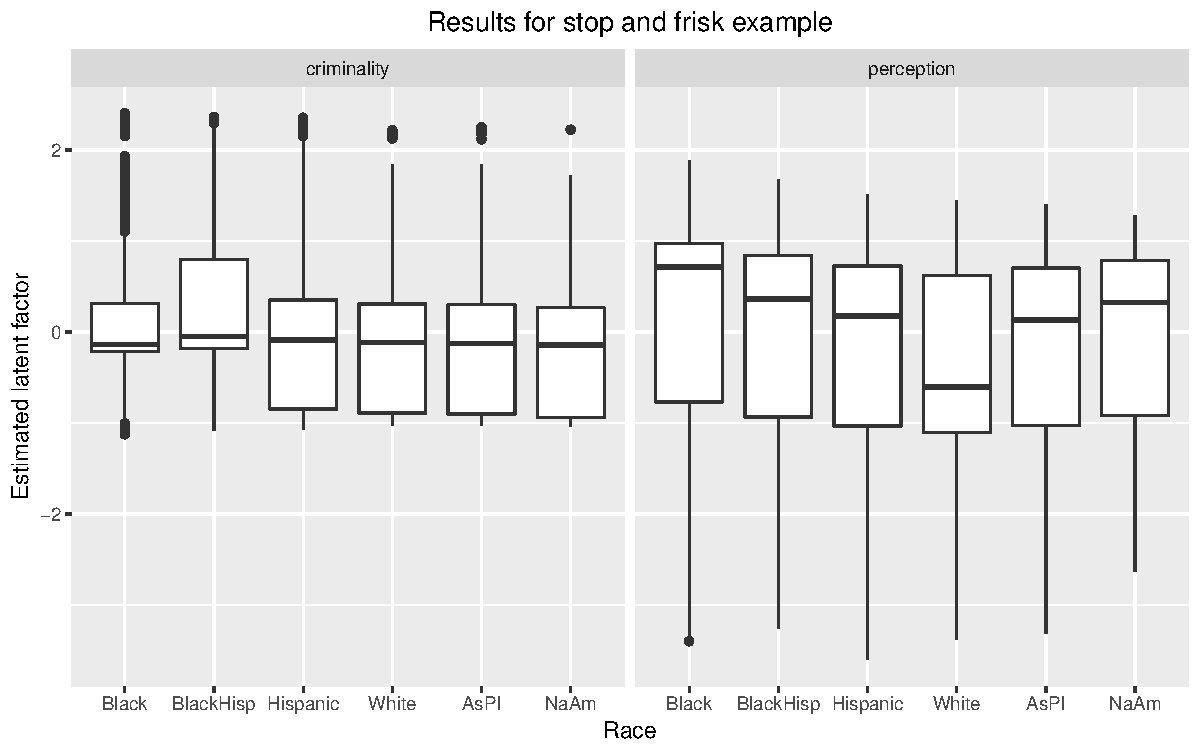
\includegraphics[width=4in]{stopandfrisk_output.pdf}}
\vspace{-2ex}
\caption{Distributions of estimated latent perception and criminality
  scores for the stop and frisk
  dataset.
\label{figure.stop_and_frisk_output}}
%\vspace{-2ex}
\end{center}
\end{figure}

Since 2002, the New York Police Department (NYPD) has recorded
information about every time a police officer has stopped someone. The
officer records information such as if the person was searched or
frisked, % if a weapon was found, their appearance, whether an arrest
was made or a summons issued, % if force was used, etc. We consider
the data collected on males stopped during 2014 which constitutes
38,609 records. % We limit our analysis to looking at just males
stopped as this accounts for more than $90\%$ of the data.  We fit a
model which decomposes these records into two latent factors, one
which depends on the race and appearance of the individual being
stopped, labeled \emph{Perceived Criminality}, and one which does not,
labeled \emph{Criminality}, and which could be used as a basis for
counterfactually fair decisions. We now describe a spatial analysis of
the estimated latent factors.

\paragraph{Model.}
We model this stop-and-frisk data using the graph in
Figure~\ref{figure.stop_and_frisk}. Specifically, we posit main causes
for the observations: \emph{Arrest} (if an individual was arrested),
\emph{Summons} (an individual was called to a court-summons),
\emph{Weapon} (an individual was found to be carrying a weapon),
\emph{Force} (some sort of force was used during the stop),
\emph{Frisked}, and \emph{Searched}. The first cause of these
observations is some measure of an individual's latent
\emph{Criminality}, which we do not observe. We believe there is an
additional cause, an individual's perceived criminality,
\emph{Perception}, also unobserved. This second factor is introduced
as we believe that these observations may be biased based on an
officer's perception of whether an individual is likely a criminal or
not. This perception is affected by an individual's \emph{Appearance}
and their \emph{Race}. In this sense \emph{Criminality} is
counterfactually fair, while \emph{Perception} models how race affects
each of the other observed variables.

\paragraph{Criminality and perception distributions.}
After fitting this model to the data we can look at the distribution
of \emph{Criminality} and \emph{Perception} across different races,
shown as box plots in Figure~\ref{figure.stop_and_frisk_output}. We see that
the median criminality for each race is nearly identical, while the
distributions are somewhat different, demonstrating that
\emph{Criminality} approaches demographic parity. The differences that
due exist may be due to unobserved confounding variables that are
affected by race or unmodeled noise in the data. On the right
\emph{Perception} varies considerably by race with white individuals
having the lowest perceived criminality while black and black Hispanic
individuals have the highest.

\begin{figure*}[!t]
\begin{center}
\centerline{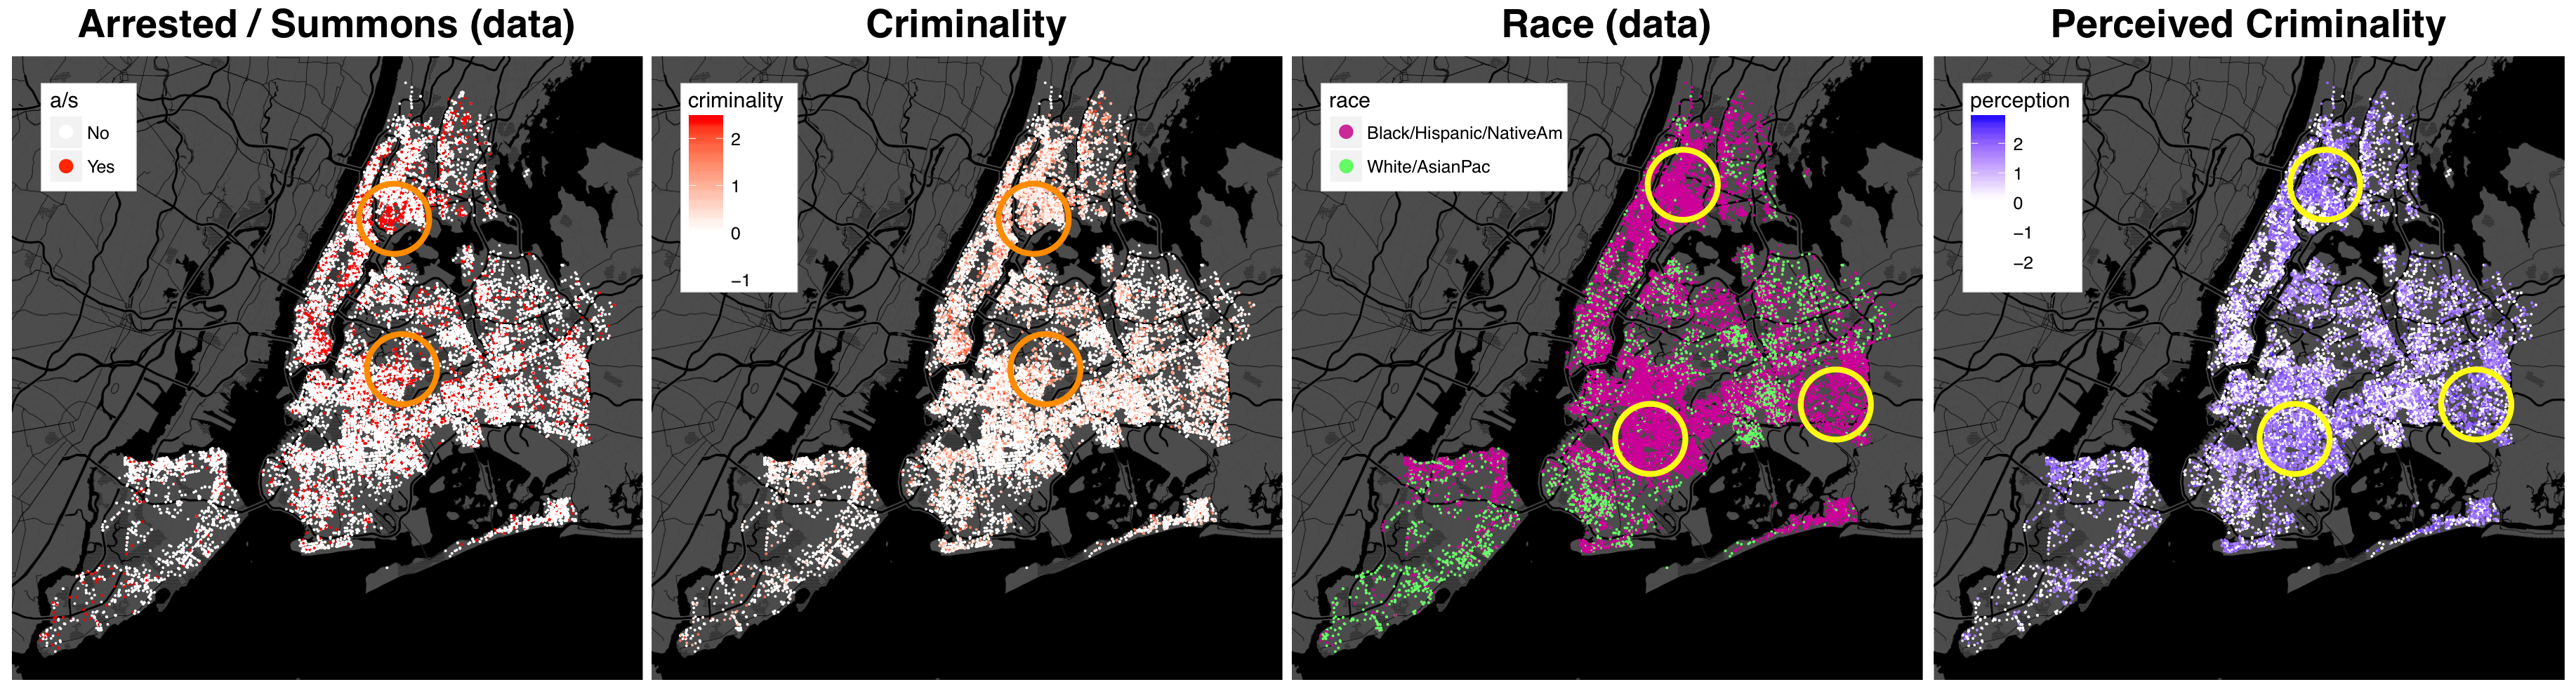
\includegraphics[width=\textwidth]{stop_and_frisk_graphs.png}}
\caption{Understanding criminality. The above maps show the
  decomposition of stop and search data in New York into factors based
  on perceived criminality (a race dependent variable) and latent
  criminality (a race neutral measure). \label{figure.criminality}}
\end{center}
\end{figure*}

\paragraph{Visualization on a map of New York City.}
Each of the stops can be mapped to longitude and latitude points for
where the stop
occurred\footnote{https://github.com/stablemarkets/StopAndFrisk}. Thus
we can visualize \emph{Criminality} and \emph{Perception} alongside
\emph{Race} and the combination of \emph{Arrest} and \emph{Summons},
shown in Figure~\ref{figure.criminality}.  Criminality seems to be a
continuous approximation of arrest and summons as both plots show red
in similar areas. However, the plots show that certain areas, while
having a lot of arrests have low criminality scores such as south
Bronx and west Queens (circled in orange). We can also compare the
perceived criminality with a plot of race, where we have divided the
races into Group A: black, black Hispanic, Hispanic, and Native
American (shown in purple); and Group B: white and Asian/Pacific
Islander (shown in green). Group A are all races that have positive
weights on the connection from \emph{Race} to \emph{Perception} in the
fitted model, while Group B all have negative weights. Thus being in
Group A leads one to have a higher perceived criminality than being in
Group B. This can be seen in the right-most plot of
Figure~\ref{figure.criminality}. Certain areas of town such as central
Brooklyn, central Bronx, and southern Queens have very high
criminality and almost all stops are by members of Group A (circled in
yellow).

%\subsection{Model criticism}
%%% Local Variables:
%%% mode: latex
%%% TeX-master: "ricardo_draft"
%%% End:


\end{document} 


% This document was modified from the file originally made available by
% Pat Langley and Andrea Danyluk for ICML-2K. This version was
% created by Lise Getoor and Tobias Scheffer, it was slightly modified  
% from the 2010 version by Thorsten Joachims & Johannes Fuernkranz, 
% slightly modified from the 2009 version by Kiri Wagstaff and 
% Sam Roweis's 2008 version, which is slightly modified from 
% Prasad Tadepalli's 2007 version which is a lightly 
% changed version of the previous year's version by Andrew Moore, 
% which was in turn edited from those of Kristian Kersting and 
% Codrina Lauth. Alex Smola contributed to the algorithmic style files.  

%%% Local Variables:
%%% mode: latex
%%% TeX-master: "ricardo_draft"
%%% End:
